% !TeX program = xelatex
% Current dataset curated-2026-10-20: 655 files, 13 classes.
% Hình minh họa nằm trong thư mục hinh/ (tạo bằng ve_hinh_minh_hoa.py).
\documentclass[11pt,a4paper]{article}
\usepackage{fontspec}
\setmainfont{texgyretermes-regular.otf}[BoldFont=texgyretermes-bold.otf,ItalicFont=texgyretermes-italic.otf,BoldItalicFont=texgyretermes-bolditalic.otf]
\setsansfont{texgyreheros-regular.otf}[BoldFont=texgyreheros-bold.otf]
\setmonofont{lmmono10-regular.otf}[Scale=0.85]
\usepackage[vietnamese]{babel}
\addto\captionsvietnamese{\renewcommand{\refname}{Tài liệu tham khảo}\renewcommand{\figurename}{Hình}\renewcommand{\tablename}{Bảng}}
\usepackage[margin=2.2cm,headheight=15pt]{geometry}
\usepackage{amsmath,amssymb,booktabs,tabularx,array,longtable,multirow}
\usepackage{graphicx,xcolor,tikz}
\graphicspath{{hinh/}{bao_cao_bo_go/hinh/}}
\usepackage{enumitem,fancyhdr,titlesec,titletoc,caption,float,needspace}
\usepackage[unicode,hidelinks]{hyperref}
\usepackage{xurl}
\titleformat{\part}[block]{\LARGE\sffamily\bfseries}{Phần \thepart.}{.5em}{}
\titlespacing*{\part}{0pt}{0pt}{14pt}
\titleformat{\section}{\Large\sffamily\bfseries}{\thesection.}{.5em}{}
\titleformat{\subsection}{\large\sffamily\bfseries}{\thesubsection}{.5em}{}
\titlespacing*{\section}{0pt}{10pt}{8pt}
\titlespacing*{\subsection}{0pt}{8pt}{4pt}
\setlength{\parindent}{0pt}
\setlength{\parskip}{5pt}
\renewcommand{\baselinestretch}{1.08}
\setlist{nosep,leftmargin=1.5em,topsep=3pt}
\renewcommand{\arraystretch}{1.18}
\captionsetup{font=small,labelfont=bf}
\pagestyle{fancy}
\fancyhf{}
\fancyhead[L]{\small\sffamily BỘ DỮ LIỆU ÂM THANH BỘ GÕ}
\fancyhead[R]{\small\sffamily Yêu cầu 1 và 2}
\fancyfoot[C]{\small\thepage}
\renewcommand{\headrulewidth}{0.3pt}
\newcommand{\note}[1]{\par\noindent\textit{#1}\par}
\hypersetup{pdftitle={Báo cáo bài tập lớn Hệ cơ sở dữ liệu đa phương tiện: tiếng nhạc cụ bộ gõ},pdfauthor={Nhóm 07}}

\setlength{\emergencystretch}{2em}
% Đặt bảng, hình ở đầu trang cùng phần chữ thay vì dồn ra trang riêng.
\renewcommand{\topfraction}{.85}\renewcommand{\textfraction}{.1}\renewcommand{\floatpagefraction}{.8}
\setcounter{tocdepth}{1}
% Phần: tiêu đề "Phần I. ..."; mục lục in hoa toàn dòng.
\newcommand{\phan}[1]{\clearpage\refstepcounter{part}\part*{Phần \thepart.\texorpdfstring{\enspace}{ }#1}}
\titlecontents{part}[0pt]{\addvspace{22pt}\sffamily\bfseries}{PHẦN \thecontentslabel.\enspace\MakeUppercase}{\MakeUppercase}{\hfill\contentspage}[\addvspace{6pt}]
\titlecontents{section}[3em]{\addvspace{8pt}}{\contentslabel[\thecontentslabel.]{1.8em}}{\hspace*{-1.8em}}{\titlerule*[.65pc]{.}\contentspage}

\begin{document}
\hypersetup{pageanchor=false}
\begin{titlepage}
\begin{tikzpicture}[remember picture,overlay]
\draw[black,line width=2pt] ([xshift=1.3cm,yshift=-1.3cm]current page.north west) rectangle ([xshift=-1.3cm,yshift=1.3cm]current page.south east);
\draw[black,line width=.6pt] ([xshift=1.5cm,yshift=-1.5cm]current page.north west) rectangle ([xshift=-1.5cm,yshift=1.5cm]current page.south east);
\end{tikzpicture}
\centering
{\large\bfseries HỌC VIỆN CÔNG NGHỆ BƯU CHÍNH VIỄN THÔNG}\par
\vspace{3pt}
{\large\bfseries KHOA CÔNG NGHỆ THÔNG TIN 1}\par
\vspace{2pt}{\rule{6cm}{.6pt}}\par
\vspace{1.2cm}

\includegraphics[height=4.4cm]{logo_ptit.png}\par
\vspace{1.3cm}
{\LARGE\bfseries BÁO CÁO BÀI TẬP LỚN}\par
\vspace{8pt}
{\LARGE\bfseries HỆ CƠ SỞ DỮ LIỆU ĐA PHƯƠNG TIỆN}\par
\vspace{1.2cm}
{\large\bfseries Đề tài:}\par
\vspace{6pt}
{\Large\bfseries XÂY DỰNG HỆ CƠ SỞ DỮ LIỆU LƯU TRỮ\\[5pt]VÀ TÌM KIẾM TIẾNG NHẠC CỤ BỘ GÕ}\par
\vspace{1.6cm}
{\large
\renewcommand{\arraystretch}{1.35}
\begin{tabular}{@{}l@{\hspace{1.5em}}l@{\hspace{2em}}l@{}}
\textbf{Lớp:} & \multicolumn{2}{l}{D23 - Lớp 04}\\
\textbf{Nhóm:} & \multicolumn{2}{l}{07}\\
\textbf{Giảng viên hướng dẫn:} & \multicolumn{2}{l}{TS. Nguyễn Đình Hóa}\\
\textbf{Thành viên nhóm:} & Hoàng Đình Kiên & B23DCCN457\\
 & Khuất Quang Minh & B23DCCN547\\
 & Nguyễn Hữu Việt & B23DCCN919\\
\end{tabular}\par}
\vfill
{\large\bfseries Hà Nội, tháng 10 năm 2026}\par
\vspace{.4cm}
\end{titlepage}
\hypersetup{pageanchor=true}
\pagenumbering{roman}

\section*{Lời nói đầu}
\pdfbookmark[1]{Lời nói đầu}{loinoidau}
Cùng với sự phát triển của Internet và các thiết bị số, dữ liệu đa phương tiện như hình ảnh, âm thanh và video chiếm tỷ trọng ngày càng lớn trong dữ liệu được lưu trữ và khai thác. Khác với văn bản hay dữ liệu có cấu trúc, dữ liệu đa phương tiện khó tìm kiếm chỉ bằng tên tệp hoặc từ khóa; việc tìm kiếm cần dựa vào chính nội dung của dữ liệu. Vì vậy, một hệ cơ sở dữ liệu đa phương tiện phải giải quyết ba bài toán: biểu diễn nội dung bằng các đặc trưng, tổ chức lưu trữ các đặc trưng đó, và tìm kiếm theo độ tương đồng.

Trong bài tập lớn này, nhóm 07 thực hiện đề tài \emph{Xây dựng hệ cơ sở dữ liệu lưu trữ và tìm kiếm tiếng nhạc cụ bộ gõ}. Âm thanh bộ gõ có những đặc điểm riêng: phần lớn nhạc cụ không có cao độ xác định, tiếng thường ngắn và năng lượng thay đổi nhanh theo thời gian. Do đó, các đặc trưng thường dùng cho tiếng nói hay âm nhạc có giai điệu cần được lựa chọn và giải thích cho phù hợp với loại âm thanh này.

Báo cáo trình bày kết quả của hai yêu cầu đầu tiên trong đề bài. Phần I mô tả bộ dữ liệu gồm 655 tệp âm thanh thuộc 13 nhóm nhạc cụ bộ gõ, cùng các điểm giống và khác nhau giữa tiếng của chúng. Phần II trình bày ba bộ đặc trưng dùng để nhận diện và tìm kiếm âm thanh tương đồng, kèm công thức, ý nghĩa và giá trị thông tin của từng đặc trưng. Các yêu cầu còn lại sẽ được xây dựng tiếp trên nền bộ dữ liệu và các bộ đặc trưng này.

Nhóm xin chân thành cảm ơn TS. Nguyễn Đình Hóa đã hướng dẫn và truyền đạt kiến thức trong suốt học phần. Do thời gian và kiến thức còn hạn chế, báo cáo khó tránh khỏi thiếu sót; nhóm rất mong nhận được ý kiến góp ý để hoàn thiện đề tài.

\vspace{1cm}
\hfill\begin{tabular}{c}
\textit{Hà Nội, tháng 10 năm 2026}\\
\textbf{Nhóm 07}
\end{tabular}
\clearpage

\section*{Đề bài}
\pdfbookmark[1]{Đề bài}{debai}
\textbf{Xây dựng hệ CSDL lưu trữ và tìm kiếm tiếng nhạc cụ bộ gõ.}
\begin{enumerate}[leftmargin=1.8em,itemsep=6pt,topsep=8pt]
\item Hãy xây dựng/sưu tầm một bộ dữ liệu âm thanh gồm ít nhất 500 files âm thanh của các nhạc cụ khác nhau thuộc bộ gõ. Các file âm thanh có độ dài phù hợp để chứa đựng đủ các đặc tính cần thiết để nhận diện tiếng nhạc cụ. Mỗi file âm thanh chỉ gồm tiếng của một nhạc cụ. Sinh viên tùy chọn định dạng file âm thanh để lưu trữ. Hãy mô tả các đặc điểm giống và khác nhau của tiếng các nhạc cụ trong các files trong bộ dữ liệu.
\item Hãy xây dựng một hoặc vài bộ đặc trưng để nhận diện âm thanh các nhạc cụ từ bộ dữ liệu đã thu thập. Các bộ thuộc tính phải bao gồm các đặc trưng giúp tìm sự tương đồng và tìm sự khác biệt giữa các âm thanh nhạc cụ trong các files dữ liệu. Hãy trình bày rõ về các đặc trưng đó và nêu giá trị thông tin của các đặc trưng được sử dụng.
\item Triển khai các thuật toán/công cụ trích rút các đặc trưng đã được xác định trong bước 2. Hãy xây dựng hệ CSDL để quản trị các đặc trưng âm thanh cho tất cả các files dữ liệu.
\item Triển khai hệ thống tìm kiếm âm thanh tương đồng với đầu vào là một file âm thanh mới về một nhạc cụ nào đó thuộc bộ gõ (nhạc cụ thuộc loại đã có và không có trong dữ liệu), đầu ra là 5 files âm thanh giống nhất, xếp thứ tự giảm dần về độ tương đồng nội dung với âm thanh đầu vào.
\begin{enumerate}[label=\alph*.,leftmargin=1.6em,itemsep=3pt,topsep=4pt]
\item Trình bày sơ đồ khối của hệ thống, chức năng của từng khối/module của hệ thống cùng các dữ liệu vào/ra cho từng khối. Mô tả quy trình thực hiện yêu cầu của đề bài.
\item Hãy minh họa các kết quả trung gian (các giá trị đặc trưng, tính toán độ tương đồng) của quá trình truy vấn âm thanh.
\item Đánh giá các kết quả đã đạt được.
\end{enumerate}
\item Demo hệ thống.
\end{enumerate}
\clearpage

\section*{Tóm tắt}
\pdfbookmark[1]{Tóm tắt}{tomtat}
Báo cáo trình bày bộ dữ liệu 655 tệp âm thanh thuộc 13 nhóm nhạc cụ bộ gõ. Các tệp được sưu tầm từ ba nguồn công khai: Freesound One-Shot Percussive Sounds, IDMT-SMT-Drums và University of Iowa Musical Instrument Samples. Mỗi tệp mang một nhãn nhạc cụ, kèm thông tin nguồn và thông số kỹ thuật. Bộ dữ liệu có cả tiếng gõ đơn lẻ và chuỗi nhiều lần gõ của cùng một nhạc cụ.

Từ bộ dữ liệu này, nhóm xây dựng ba bộ đặc trưng: \textbf{bộ A gồm 21 thuộc tính về thời gian và phổ}, \textbf{bộ B gồm 39 thuộc tính MFCC} và \textbf{bộ C ghép A với B thành 60 thuộc tính}. Mỗi tệp âm thanh được biến thành một vector số. Vector này cho biết năng lượng của âm thay đổi theo thời gian ra sao và nằm ở những vùng tần số nào, chẳng hạn âm trầm hay sáng, phổ tập trung hay trải rộng. Hai âm thanh càng giống nhau thì khoảng cách Euclid giữa hai vector (sau khi chuẩn hóa) càng nhỏ. Đây là cơ sở để lưu trữ và tìm kiếm âm thanh tương đồng ở các yêu cầu sau.

\begin{table}[htbp]
\centering\small
\caption{Đối chiếu nội dung đề bài với các phần của báo cáo.}\label{tab:doichieu}
\begin{tabularx}{\textwidth}{p{.3\textwidth}X}
\toprule
Nội dung đề bài & Nội dung đáp ứng trong báo cáo\\\midrule
Ít nhất 500 tệp bộ gõ & 655 tệp: nguồn, tổ chức và kiểm tra, Mục~\ref{sec:nguon}--\ref{sec:curation}.\\
Độ dài phù hợp; một nhạc cụ mỗi tệp & Tiêu chí tuyển chọn, phân tích thời lượng và cách bảo đảm mỗi tệp chỉ có một nhạc cụ, Mục~\ref{sec:curation}--\ref{sec:quymo}.\\
Tự chọn định dạng lưu trữ & WAV PCM 16-bit mono 16 kHz và lý do chọn, Mục~\ref{sec:dinhdang}.\\
Mô tả điểm giống và khác nhau & Phân loại 13 nhóm, phổ đồ, bảng mô tả và số đo trực tiếp, Mục~\ref{sec:dacdiem}--\ref{sec:dinhluong}.\\
Xây dựng một hoặc vài bộ đặc trưng & Quy trình và công thức của ba bộ A, B, C, Mục~\ref{sec:quytrinh}--\ref{sec:boC}.\\
Đặc trưng tìm tương đồng và khác biệt & Phép đo khoảng cách và vai trò từng nhóm thuộc tính, Mục~\ref{sec:boC} và \ref{sec:dongop}.\\
Giá trị thông tin của đặc trưng & Giải thích từng thuộc tính và kết quả định lượng trên dữ liệu, Mục~\ref{sec:boA-tg}--\ref{sec:dongop}.\\\bottomrule
\end{tabularx}
\end{table}
\clearpage
\pdfbookmark[1]{Mục lục}{mucluc}
{\centering\sffamily\bfseries\LARGE MỤC LỤC\par}
\vspace{18pt}
\makeatletter\@starttoc{toc}\makeatother
\clearpage
\pagenumbering{arabic}

\phan{Yêu cầu 1: Bộ dữ liệu âm thanh nhạc cụ bộ gõ}
\section{Đối tượng, nguồn và định dạng dữ liệu}\label{sec:nguon}
\subsection{Đối tượng, đơn vị dữ liệu và nhãn}
Đối tượng của bộ dữ liệu là âm thanh của các nhạc cụ bộ gõ. Mỗi bản ghi trong bộ dữ liệu là \textbf{một tệp WAV}, và đây cũng là đơn vị được trả về khi tìm kiếm. Mỗi tệp có đúng một nhãn cho biết đó là nhạc cụ nào trong 13 nhóm. Nhãn không ghi người chơi, cao độ hay kỹ thuật đánh. Trong báo cáo, mỗi nhóm nhạc cụ còn được gọi là một \emph{lớp}, theo cách gọi quen thuộc trong phân loại dữ liệu. Bảng~\ref{tab:phanloai} chia 13 nhóm thành bốn họ theo cách nhạc cụ tạo ra âm thanh, và các phần so sánh về sau đều dùng cách chia này.

\begin{table}[htbp]
\centering\small
\caption{Phân loại 13 nhóm nhạc cụ trong bộ dữ liệu theo cách tạo âm.}\label{tab:phanloai}
\begin{tabularx}{\textwidth}{p{.33\textwidth}p{.3\textwidth}X}
\toprule
Họ nhạc cụ & Nhãn trong bộ dữ liệu & Nguồn rung chính\\\midrule
Màng rung (membranophone) & kick, tom, conga, snare & Mặt trống; snare có thêm dây lò xo dưới mặt trống.\\
Tự thân vang, kim loại, không có cao độ xác định & hi-hat, cymbal, cowbell, agogo, tambourine & Thân kim loại; tambourine có các miếng chũm chọe nhỏ, một số mẫu có cả mặt màng.\\
Tự thân vang, gỗ, không có cao độ xác định & claves & Hai thanh gỗ gõ vào nhau.\\
Thanh gõ có cao độ xác định & marimba, xylophone, vibraphone & Thanh gỗ (marimba, xylophone) hoặc thanh kim loại (vibraphone) được lên dây theo nốt.\\\bottomrule
\end{tabularx}
\end{table}

\textbf{Cách gán nhãn.} Nhãn được gán dựa trên tên tệp và thông tin mô tả (metadata) do nguồn cung cấp:
\begin{itemize}
\item Freesound: dựa trên tên và mô tả của âm thanh, ví dụ tệp ``crash mute1.wav'' được xếp vào nhóm cymbal.
\item IDMT: dựa trên mã nhạc cụ trong tên tệp, gồm \texttt{KD} là kick, \texttt{SD} là snare và \texttt{HH} là hi-hat.
\item Iowa: dùng tên nhạc cụ do thư viện ghi sẵn.
\end{itemize}
Sau đó, nhãn được xác minh và sàng lọc lại theo các bước ở Mục~\ref{sec:curation}.

Yêu cầu ``mỗi tệp chỉ gồm tiếng của một nhạc cụ'' không có nghĩa là mỗi tệp chỉ có một lần gõ. Một tệp hi-hat đánh nhiều lần liên tiếp vẫn hợp lệ, miễn là trong tệp chỉ có tiếng hi-hat. Tương tự, tiếng snare gồm tiếng thân trống và tiếng rè của dây lò xo, nhưng cả hai đều do cùng một chiếc trống tạo ra. Trường hợp không hợp lệ là bản phối có nhiều nhạc cụ cùng chơi.

\subsection{Nguồn sưu tầm}
\begin{table}[htbp]
\centering\small
\caption{Ba nguồn dữ liệu và số tệp lấy từ mỗi nguồn.}\label{tab:nguon}
\begin{tabularx}{\textwidth}{p{.27\textwidth}rX}
\toprule
Nguồn & Số tệp & Nhãn và cách xác minh\\\midrule
Freesound One-Shot Percussive Sounds~\cite{freesound} & 513 & 11 nhóm (trừ marimba, vibraphone). Đối chiếu mã âm thanh, tên và người tải lên với metadata chính thức.\\
IDMT-SMT-Drums~\cite{idmt} & 94 & 54 hi-hat, 32 kick, 8 snare; gồm 56 tệp thuộc phần training của IDMT và 38 rãnh tách riêng từng nhạc cụ (isolated tracks). Đối chiếu dạng sóng với gói chính thức.\\
University of Iowa MIS~\cite{iowa} & 48 & 36 marimba, 12 vibraphone; đoạn trích từ các bản thu theo nốt của thư viện.\\\midrule
\textbf{Tổng} & \textbf{655} & Ba nguồn bổ sung độ đa dạng về nhạc cụ và điều kiện thu.\\\bottomrule
\end{tabularx}
\end{table}
Freesound One-Shot Percussive Sounds là tập tiếng bộ gõ, mỗi tệp là một lần gõ (one-shot), đã được các tác giả của tập dữ liệu sàng lọc~\cite{freesound}. IDMT có cả bản phối trống lẫn bản thu riêng từng nhạc cụ; nhóm chỉ lấy các bản thu riêng, không lấy bản phối~\cite{idmt}. Thư viện Iowa sắp xếp mẫu theo nhạc cụ, cao độ, cường độ và kỹ thuật chơi~\cite{iowa}.

\subsection{Định dạng và tổ chức lưu trữ}\label{sec:dinhdang}
Mọi tệp đều có cùng một định dạng: WAV PCM 16-bit, một kênh (mono), tần số lấy mẫu 16.000 Hz. Nhóm chọn WAV PCM vì đây là định dạng không nén: lưu lại không làm mất thông tin, đọc được bằng hầu hết thư viện xử lý âm thanh và thuận tiện khi tính đặc trưng.

Một số nguồn thu ở tần số lấy mẫu cao hơn, ví dụ IDMT là 44,1 kHz. Khi đưa về 16 kHz, mọi thành phần trên 8 kHz (một nửa tần số lấy mẫu, gọi là tần số Nyquist) bị loại bỏ. Dải 0--8 kHz đủ để thấy phần lớn khác biệt giữa các nhạc cụ trong bộ dữ liệu, nhưng tiếng kim loại như cymbal, hi-hat và tambourine bị mất một phần âm cao. Âm thanh truy vấn ở các yêu cầu sau cũng phải được đưa về đúng định dạng này trước khi tính đặc trưng (Mục~\ref{sec:sudung}).

Các tệp được xếp vào 13 thư mục, mỗi thư mục ứng với một nhãn. Đi kèm các tệp âm thanh là ba loại bảng dữ liệu:
\begin{itemize}
\item \textbf{Bảng danh mục:} mỗi tệp một dòng, gồm mã tệp, đường dẫn, nhãn, nguồn, người tải lên và mã băm SHA-256. Mã băm là một chuỗi ký tự tính từ nội dung tệp, dùng để phát hiện tệp trùng nhau hoặc tệp đã bị thay đổi.
\item \textbf{Bảng kiểm kê:} thời lượng và kết quả kiểm tra tín hiệu của từng tệp.
\item \textbf{Bảng đặc trưng:} giá trị các thuộc tính của bộ A, B, C cho từng tệp.
\end{itemize}
Các bảng liên kết với nhau qua mã tệp, và đây cũng là phần dữ liệu sẽ được đưa vào hệ cơ sở dữ liệu ở Yêu cầu 3. Tên tệp và thông tin nguồn chỉ dùng để quản lý, \textbf{không được đưa vào vector đặc trưng}.

\section{Tuyển chọn và kiểm soát chất lượng}\label{sec:curation}
Một tệp chỉ được đưa vào bộ dữ liệu khi đạt cả năm bước kiểm tra dưới đây, và cả \textbf{655 tệp} đều đạt. Các ngưỡng số trong từng bước do nhóm tự đặt ra để bảo đảm chất lượng, đề bài không quy định.
\begin{enumerate}
\item \textbf{Kiểm kê và loại trùng:} đọc từng tệp, đối chiếu nhãn với thư mục chứa tệp, rồi tính mã SHA-256 cho cả tệp và cho phần dữ liệu âm thanh bên trong (chuỗi mẫu PCM). Không có hai tệp nào trùng mã. Cách này chỉ phát hiện được hai tệp giống hệt nhau, chưa phát hiện được hai bản thu gần giống nhau.
\item \textbf{Kiểm tra tín hiệu:} tệp phải thỏa mãn tất cả các điều kiện sau.
\begin{itemize}
\item Đọc được, không rỗng và không chứa giá trị lỗi (không xác định hoặc vô hạn).
\item Dài ít nhất 0,1 s, trong đó phần có tiếng dài ít nhất 0,05 s.
\item Đủ to: mẫu có biên độ lớn nhất không thấp hơn $-40$ dBFS. dBFS là mức âm tính theo decibel so với mức lớn nhất mà định dạng lưu được.
\item Không bị cắt mất phần đầu tiếng gõ: biên độ của mẫu đầu tiên không quá 10\% biên độ lớn nhất.
\item Không bị cắt cụt ở cuối tệp và không bị méo do vượt mức ghi (clipping).
\end{itemize}
\item \textbf{Xác minh nguồn và nhãn:} mỗi tệp phải có thông tin nguồn, và các quy tắc gán nhãn không được cho ra hai nhạc cụ khác nhau cho cùng một tệp. Với Freesound, nhóm đối chiếu với metadata chính thức của tập dữ liệu. Với IDMT, nhóm so sánh dạng sóng của từng tệp với tệp gốc trong gói chính thức, sau khi đưa về cùng tần số lấy mẫu. Cả 94 tệp đều có độ tương đồng cosine trên 0,99, tức gần như trùng khớp với bản gốc.
\item \textbf{Sàng lọc nội dung:} không đưa vào bộ dữ liệu những tệp có dấu hiệu tiếng nói, nhiều nhạc cụ cùng chơi hoặc hiệu ứng nhiễu, và những tệp có nhãn không khớp với nội dung âm thanh.
\item \textbf{Cân đối nhóm và chốt phiên bản:} mỗi nhóm nhạc cụ phải có ít nhất 5 tệp đạt chuẩn. Sau đó, danh sách 655 tệp được cố định. Mọi số liệu, tham số chuẩn hóa và đặc trưng trong báo cáo đều được tính trên đúng 655 tệp này.
\end{enumerate}

\section{Quy mô, thời lượng và độ phù hợp của tệp}\label{sec:quymo}
\begin{table}[htbp]
\centering
\caption{Số lượng và thời lượng đo trực tiếp trên phiên bản 655 tệp. Đơn vị thời lượng: giây.}\label{tab:thoiluong}
\begin{tabular}{lrrrr}
\toprule
Nhãn nhạc cụ & Số tệp & Ngắn nhất & Trung vị & Dài nhất\\\midrule
agogo & 16 & 0,464 & 0,673 & 0,999 \\
claves & 13 & 0,163 & 0,209 & 0,511 \\
conga & 18 & 0,139 & 0,476 & 0,906 \\
cowbell & 43 & 0,110 & 0,232 & 0,720 \\
cymbal & 33 & 0,371 & 0,766 & 0,999 \\
hi-hat & 93 & 0,108 & 5,647 & 19,249 \\
kick & 151 & 0,109 & 0,480 & 20,615 \\
marimba & 36 & 0,712 & 2,000 & 2,000 \\
snare & 141 & 0,114 & 0,464 & 17,104 \\
tambourine & 12 & 0,154 & 0,395 & 0,418 \\
tom & 76 & 0,107 & 0,720 & 0,999 \\
vibraphone & 12 & 2,000 & 2,000 & 2,000 \\
xylophone & 11 & 0,283 & 0,510 & 0,958 \\
\midrule
\textbf{Tổng} & \textbf{655} & \textbf{0,107} & \textbf{0,534} & \textbf{20,615}\\\bottomrule
\end{tabular}
\end{table}
Tổng thời lượng của bộ dữ liệu là \textbf{1.583,158 giây} (khoảng 26 phút 23 giây), tổng dung lượng là 50.689.868 byte (khoảng 48,34 MiB). Phần lớn tệp rất ngắn: 514 tệp dài không quá 1 giây. Số tệp giữa các lớp chênh lệch nhiều, từ 11 tệp (xylophone) đến 151 tệp (kick).

\subsection{Vì sao không ép mọi tệp về cùng độ dài}
Đề bài yêu cầu mỗi tệp có ``độ dài phù hợp'' để chứa đủ đặc tính nhận diện nhạc cụ. Với bộ gõ, những phần có ích để nhận diện là lúc tiếng gõ bắt đầu (khởi âm), phần ngân (cộng hưởng) và cách tiếng nhỏ dần hoặc lặp lại. Vì vậy, độ dài phù hợp khác nhau giữa các nhạc cụ. Tiếng claves hay cowbell vốn rất ngắn, nên thêm im lặng cho dài ra không mang thêm thông tin. Ngược lại, nếu cắt chuỗi hi-hat hay tiếng ngân dài về cùng một độ dài ngắn thì sẽ mất các đặc điểm về thời gian.

Do đó, nhóm giữ nguyên độ dài gốc của từng tệp. Khi tính đặc trưng, mỗi tệp dù dài hay ngắn đều được tóm tắt thành một vector có cùng số chiều (Mục~\ref{sec:quytrinh}), nên vẫn so sánh được với nhau. Ngưỡng 0,1 s ở Mục~\ref{sec:curation} chỉ để loại tệp lỗi. Một tệp có phù hợp hay không còn tùy vào tốc độ tắt dần của tiếng, việc tệp có bị cắt cụt ở đầu hoặc cuối hay không, và cách chơi, chứ không chỉ tùy vào thời lượng.

\subsection{Ảnh hưởng của dạng bản ghi}
Bộ dữ liệu có hai dạng bản ghi: tiếng gõ đơn và chuỗi nhiều lần gõ. Có 92 tệp dài hơn 2 s, và tất cả đều là chuỗi nhiều lần gõ lấy từ IDMT, gồm 53 hi-hat, 31 kick và 8 snare. Riêng các tệp hi-hat đã chiếm khoảng 700 s, gần một nửa tổng thời lượng. Vì vậy, tệp hi-hat dài hơn tệp claves không có nghĩa là một tiếng hi-hat ngân lâu hơn một tiếng claves; tệp hi-hat dài chỉ vì chứa nhiều lần đánh. Nói chung, thời lượng của tệp phụ thuộc cả vào cách cắt, số lần đánh và khoảng nghỉ, chứ không chỉ vào độ ngân của nhạc cụ. Mục~\ref{sec:sodo} đo ảnh hưởng của dạng bản ghi lên khoảng cách đặc trưng.

Các đoạn lấy từ Iowa được cắt dài tối đa 2 s. Cả 12 tệp vibraphone và 33/36 tệp marimba dài đúng 2 s, nghĩa là phần cuối của tiếng ngân bị cắt bớt. Tuy vậy, như Hình~\ref{fig:pho} cho thấy, phần đầu tiếng gõ và đoạn đầu lúc tiếng nhỏ dần vẫn còn, đủ để thấy các vạch tần số đặc trưng của hai nhạc cụ.

\section{Đặc điểm giống và khác nhau của tiếng nhạc cụ}\label{sec:dacdiem}
\subsection{Những đặc điểm chung}
Mọi tiếng bộ gõ đều có chung một diễn biến: nhạc cụ bị gõ trong một khoảnh khắc rất ngắn (kích thích), sau đó rung lên (cộng hưởng) rồi tắt dần. Một tệp có thể chứa nhiều lần gõ như vậy. Xét theo tần số, mỗi tiếng gồm hai thành phần: các vạch tần số rõ rệt, và phần năng lượng trải rộng trên nhiều tần số, nghe giống tiếng xì của nhiễu. Tỷ lệ giữa hai thành phần này khác nhau tùy nhạc cụ. Vật liệu, cấu tạo, chỗ gõ, lực gõ và cách hãm tiếng làm cho các nhạc cụ khác nhau về độ trầm, độ sáng, độ rè và thời gian ngân.

Hai tệp của cùng một nhạc cụ không nhất thiết giống hệt nhau, còn hai nhạc cụ khác nhau lại có thể giống nhau ở một số mặt. Ví dụ, kick, conga và tom đều có nhiều năng lượng ở tần số thấp (tiếng trầm), còn hi-hat và tambourine đều có nhiều năng lượng ở tần số cao (tiếng sáng). Vì vậy, không thể nhận diện nhạc cụ chỉ bằng một chỉ số duy nhất, mà cần nhiều thuộc tính bổ sung cho nhau.

\subsection{Quan sát trên phổ đồ}
Hình~\ref{fig:pho} vẽ dạng sóng và phổ đồ của một tệp đại diện cho mỗi nhóm. Dạng sóng cho thấy biên độ thay đổi theo thời gian. Phổ đồ cho thấy năng lượng nằm ở những tần số nào tại từng thời điểm: trục ngang là thời gian, trục dọc là tần số, màu càng đậm thì năng lượng càng lớn. Tệp đại diện là tệp có thời lượng và trọng tâm phổ (Mục~\ref{sec:boA-pho}) gần với giá trị trung vị của nhóm nhất, so sánh trên thang logarit. Phổ đồ dùng cùng cách chia khung với bộ đặc trưng: khung 25 ms, bước 10 ms, FFT 512 điểm.

\begin{figure}[htbp]
\centering
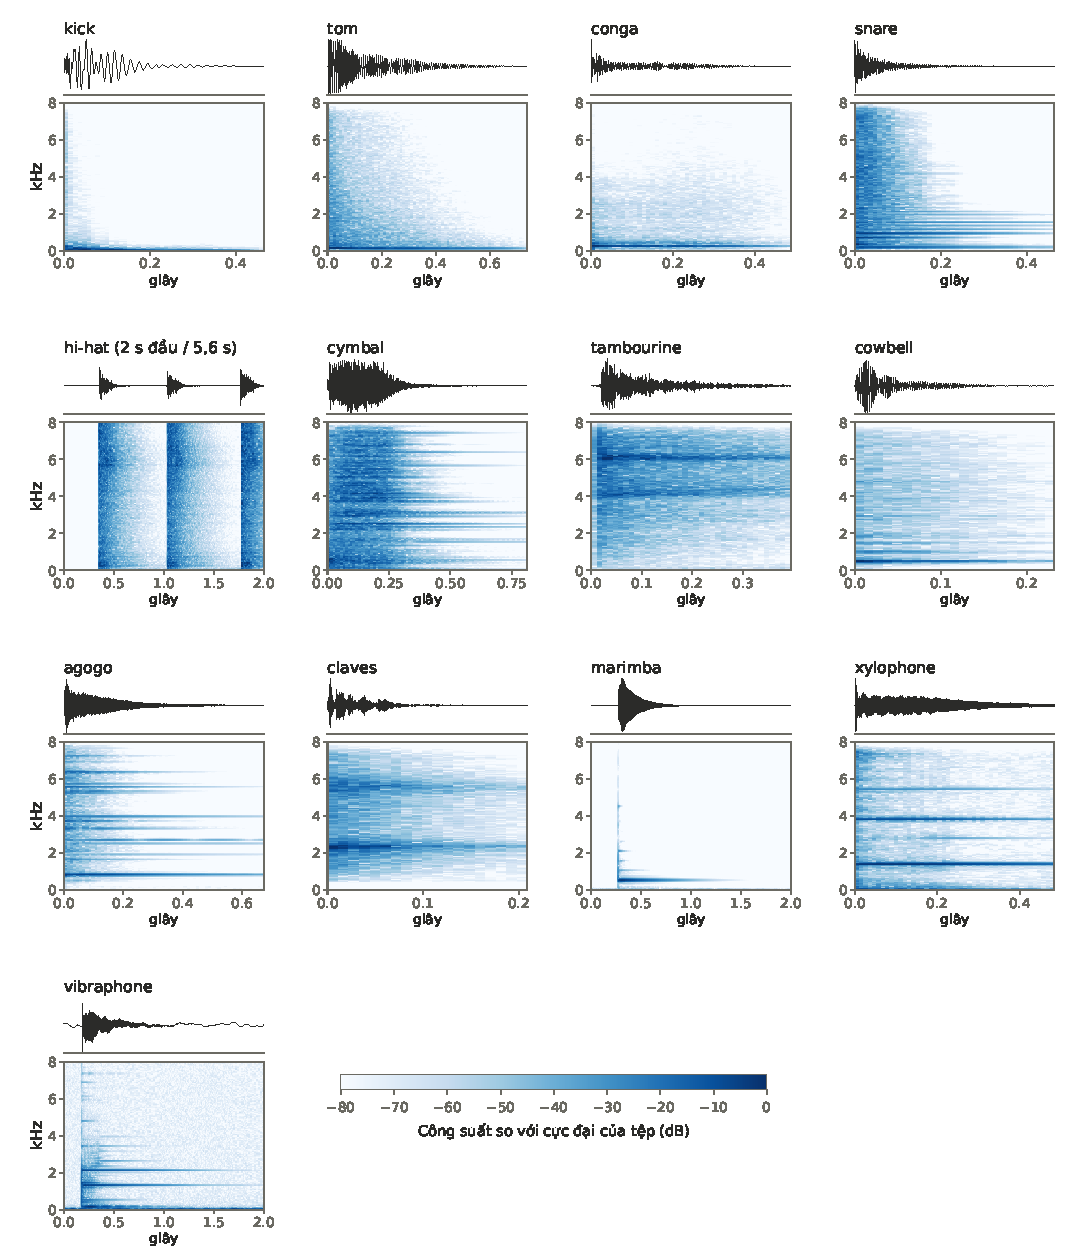
\includegraphics[width=\textwidth]{hinh1_song_va_pho.pdf}
\caption{Dạng sóng (trên) và phổ đồ 0--8 kHz (dưới) của tệp đại diện mỗi nhóm, xếp theo họ nhạc cụ ở Bảng~\ref{tab:phanloai}. Tệp hi-hat lấy từ IDMT, marimba và vibraphone lấy từ Iowa, các tệp còn lại lấy từ Freesound. Mỗi ô có trục thời gian riêng theo độ dài tệp, tối đa 2 s; tệp hi-hat là chuỗi nhiều lần đánh nên chỉ vẽ 2 s đầu. Màu đậm là công suất gần cực đại của tệp. Năng lượng của kick, tom, conga tập trung dưới 0,5 kHz nên chỉ chiếm dải hẹp ở đáy phổ đồ.}\label{fig:pho}
\end{figure}

Các điểm giống và khác nhau nhìn thấy được trên Hình~\ref{fig:pho}:
\begin{itemize}
\item \textbf{Trống màng rung trầm (kick, tom, conga):} năng lượng dồn vào vài vạch tần số thấp. Trên tệp đại diện, phổ trung bình có đỉnh ở khoảng 52 Hz với kick, 122 Hz với tom, và ở 232 Hz cùng 393 Hz với conga. Ngoài các vạch này chỉ có một vệt dọc rất ngắn lúc vừa gõ, trải trên nhiều tần số. Tom ngân lâu hơn kick và conga.
\item \textbf{Snare:} giống ba trống trên ở các vạch dưới 1,5 kHz do thân trống tạo ra. Điểm khác là trong khoảng 0,2 s đầu có thêm một vùng năng lượng giống nhiễu trải tới 8 kHz, do dây lò xo rung.
\item \textbf{Hi-hat và cymbal:} cả hai đều có năng lượng dày đặc, phủ gần hết dải 0--8 kHz. Hai nhạc cụ khác nhau ở thời gian: cymbal ngân lâu với nhiều vạch đan xen, còn mỗi lần đánh hi-hat chỉ là một vệt dọc ngắn, lặp lại theo nhịp.
\item \textbf{Tambourine:} cũng sáng như hi-hat, nhưng năng lượng không trải đều mà dồn vào hai dải hẹp quanh 4,1--4,8 kHz và 6,1--6,3 kHz, kéo dài suốt tệp.
\item \textbf{Cowbell và agogo:} đều là chuông kim loại với vài vạch tần số rời rạc. Vạch của cowbell nằm thấp (khoảng 0,48 và 1,0 kHz) và tắt nhanh. Vạch của agogo cao hơn (khoảng 0,8; 2,7; 4,0 và 5,6 kHz) và ngân lâu hơn.
\item \textbf{Claves:} rất ngắn (khoảng 0,2 s), năng lượng tập trung ở hai cụm quanh 2,1--2,5 kHz và 5,5--5,8 kHz.
\item \textbf{Marimba, xylophone, vibraphone:} cả ba đều có các vạch nằm ngang rõ nét, vì mỗi thanh gõ được chỉnh để phát ra một nốt nhạc xác định. Marimba gần như chỉ có một vạch chính (khoảng 0,53 kHz, gần nốt C5). Xylophone có các vạch ở 1,4 và 3,8 kHz. Vibraphone có các vạch dưới 2,2 kHz, ngân suốt 2 s.
\end{itemize}

\subsection{Mô tả 13 nhóm và các dấu hiệu so sánh}
Bảng~\ref{tab:mota} tóm tắt đặc điểm của từng nhóm và nhóm dễ bị nhầm với nó. Nội dung bảng dựa trên cấu tạo nhạc cụ, phổ đồ ở Hình~\ref{fig:pho} và số đo ở Mục~\ref{sec:dinhluong}. Đây là đặc điểm chung của cả nhóm, còn từng tệp cụ thể có thể khác đi tùy cách chơi và cách xử lý bản thu.
\begin{table}[htbp]
\centering\small
\caption{Đặc điểm của 13 nhóm nhạc cụ và nhóm dễ nhầm lẫn với chúng.}\label{tab:mota}
\begin{tabularx}{\textwidth}{p{.15\textwidth}X}
\toprule
Nhạc cụ & Đặc điểm và điểm so sánh đáng chú ý\\\midrule
Kick & Thân tiếng rất trầm, xung năng lượng mạnh và tắt nhanh. Gần tom và conga ở năng lượng thấp; khác ở vị trí vạch trầm và diễn biến năng lượng.\\
Tom & Cộng hưởng mặt trống, có thân tiếng và đuôi suy giảm dài hơn kick. Gần conga nhất trong bộ dữ liệu.\\
Conga & Trống tay; tiếng thay đổi theo cách đánh mở, hãm hoặc vỗ. Phần trầm gần tom, phần đầu tiếng thay đổi mạnh theo kỹ thuật.\\
Snare & Thân tiếng trống kết hợp phần rè của dây lò xo, nên phổ phân tán hơn các trống trầm và gần cymbal ở thành phần nhiễu.\\
Hi-hat & Tiếng kim loại sáng, phổ gần giống nhiễu; đóng hay mở tạo độ ngân khác nhau. Gần tambourine về độ sáng, gần cymbal và snare về độ phân tán.\\
Cymbal & Nhiều thành phần kim loại, phổ trải rộng, đuôi ngân dài. Có chung tính nhiễu với hi-hat và snare.\\
Tambourine & Các miếng kim loại nhỏ tạo tiếng leng keng ở dải cao, tập trung vào vài dải hẹp. Trọng tâm phổ cao nhất bộ dữ liệu.\\
Cowbell & Chuông kim loại với vài vạch cộng hưởng thấp, tắt nhanh. Cùng kiểu vạch rời rạc với agogo nhưng vạch nằm thấp hơn.\\
Agogo & Chuông gõ với các vạch cộng hưởng rời rạc ở dải trung và cao; cỡ chuông và lực đánh làm dịch vạch. Phân biệt với cowbell nhờ vị trí vạch.\\
Claves & Va chạm hai thanh gỗ, rất ngắn và sắc, năng lượng tập trung ở vài kHz. Khởi âm rõ như nhiều nhạc cụ khác nhưng đuôi tiếng ngắn nhất.\\
Marimba & Thanh gỗ có cao độ, có ống cộng hưởng; năng lượng dồn vào vạch cơ bản, vạch cao tắt nhanh. Cao độ nốt làm dịch toàn bộ phổ.\\
Vibraphone & Thanh kim loại có cao độ, ngân dài nếu không hãm tiếng. Gần marimba về độ tập trung phổ.\\
Xylophone & Thanh gỗ có cao độ, âm sáng và khởi âm rõ. Trong bộ dữ liệu có trọng tâm phổ cao hơn hẳn marimba và vibraphone.\\\bottomrule
\end{tabularx}
\end{table}

\section{So sánh định lượng tiếng nhạc cụ}\label{sec:dinhluong}
\subsection{Cách đọc số liệu}
Mục này dùng số đo để kiểm chứng những gì quan sát được ở Mục~\ref{sec:dacdiem}. Mỗi tệp được chia thành nhiều khung ngắn 25 ms. Mỗi đại lượng được tính trên từng khung có tiếng, rồi lấy trung bình cho cả tệp. Bảng~\ref{tab:acoustic} ghi \textbf{trung vị} của các giá trị trung bình đó trong mỗi lớp, tức giá trị nằm ở giữa khi xếp các tệp của lớp theo thứ tự. Trung vị cho biết giá trị tiêu biểu của lớp, nhưng không cho biết các tệp trong lớp khác nhau nhiều hay ít. Ý nghĩa ngắn gọn của các đại lượng như sau, còn công thức nằm ở Mục~\ref{sec:quytrinh}--\ref{sec:boA-pho}:
\begin{itemize}
\item $C$ (trọng tâm phổ): âm trầm hay sáng; giá trị càng lớn thì âm càng sáng.
\item $F$ (độ phẳng phổ) và $H$ (entropy phổ): phổ dồn vào vài vạch (giá trị nhỏ) hay trải đều trên nhiều tần số giống nhiễu (giá trị lớn).
\item $L$: phần năng lượng nằm dưới 500 Hz, tức mức độ ``trầm'' của âm.
\item $\Phi$ (thông lượng phổ): phổ thay đổi nhanh hay chậm giữa các khung liên tiếp.
\end{itemize}
\begin{table}[H]
\centering\small
\caption{Các đại lượng phổ đo trên bộ dữ liệu (trung vị theo lớp). $C$: trọng tâm phổ; $F$: độ phẳng phổ; $H$: entropy phổ; $L$: tỷ lệ năng lượng dưới 500 Hz; $\Phi$: thông lượng phổ.}\label{tab:acoustic}
\begin{tabular}{lrrrrr}
\toprule
Nhãn & $C$ (Hz) & $F$ & $H$ & $L$ (\%) & $\Phi$\\\midrule
agogo & 1.261,3 & 0,0015 & 0,272 & $<0{,}01$ & 0,045 \\
claves & 2.668,7 & 0,0121 & 0,458 & $<0{,}01$ & 0,363 \\
conga & 240,6 & 0,0001 & 0,256 & 99,61 & 0,117 \\
cowbell & 720,6 & 0,0036 & 0,252 & 42,04 & 0,141 \\
cymbal & 2.838,4 & 0,0910 & 0,710 & 3,38 & 0,338 \\
hi-hat & 4.429,7 & 0,2945 & 0,839 & 9,23 & 0,403 \\
kick & 60,3 & 0,0002 & 0,229 & 99,84 & 0,188 \\
marimba & 245,2 & 0,0002 & 0,219 & 78,91 & 0,059 \\
snare & 1.749,6 & 0,1661 & 0,696 & 29,89 & 0,353 \\
tambourine & 5.766,8 & 0,0211 & 0,584 & 0,01 & 0,397 \\
tom & 144,0 & 0,0007 & 0,234 & 99,20 & 0,088 \\
vibraphone & 307,9 & 0,0003 & 0,198 & 76,85 & 0,053 \\
xylophone & 1.889,3 & 0,0003 & 0,254 & 5,85 & 0,070 \\
\bottomrule
\end{tabular}
\end{table}

\begin{figure}[H]
\centering
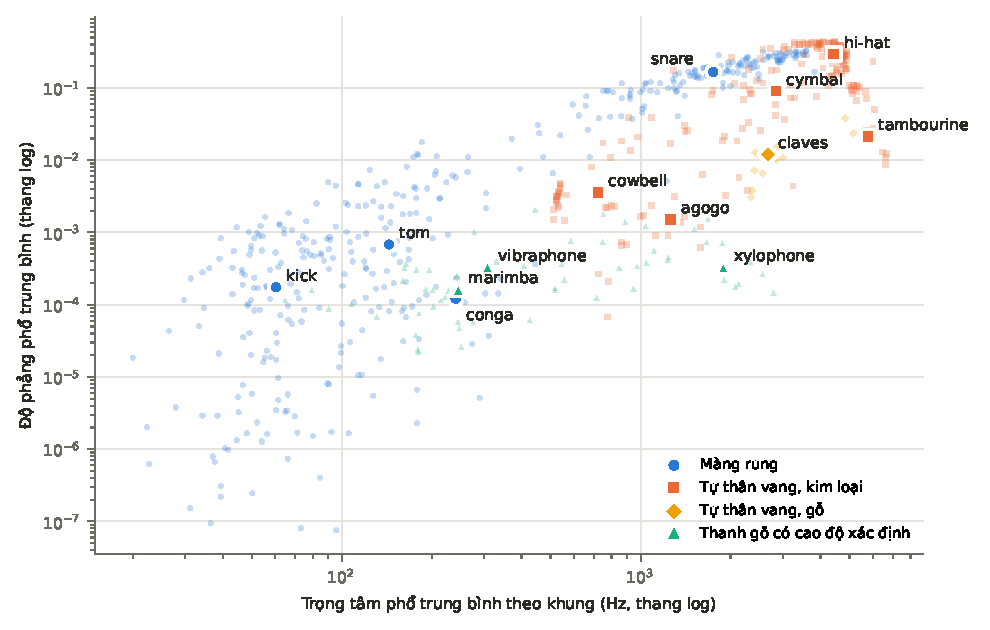
\includegraphics[width=.92\textwidth]{hinh2_trong_tam_do_phang.pdf}
\caption{Trọng tâm phổ và độ phẳng phổ của 655 tệp (điểm nhạt) và trung vị từng lớp (điểm đậm có nhãn), tô màu và phân biệt hình dạng điểm theo bốn họ nhạc cụ ở Bảng~\ref{tab:phanloai}. Cả hai trục dùng thang logarit.}\label{fig:phantan}
\end{figure}

\subsection{Những tương đồng và khác biệt quan sát được}
\textbf{Nhóm trống trầm:} kick, tom và conga có tỷ lệ năng lượng dưới 500 Hz lần lượt là 99,84\%, 99,20\% và 99,61\%, tức gần như toàn bộ năng lượng nằm ở dải trầm. Đây là điểm giống nhau rõ nhất của ba nhạc cụ. Tuy vậy, trọng tâm phổ của chúng khác nhau (khoảng 60,3; 144,0 và 240,6 Hz), nghĩa là trong dải trầm, kick trầm nhất và conga cao nhất. Trên Hình~\ref{fig:phantan}, ba lớp cùng nằm ở góc trái phía dưới, và các điểm của từng tệp chồng lên nhau khá nhiều.

\textbf{Nhóm phổ phân tán:} entropy của hi-hat là 0,839, cymbal 0,710 và snare 0,696, cao hơn hẳn nhóm trống trầm (0,229--0,256). Nghĩa là năng lượng của ba nhạc cụ này trải trên nhiều tần số. Hi-hat và tambourine đều sáng, với trọng tâm phổ khoảng 4.429,7 và 5.766,8 Hz. Nhưng độ phẳng của hi-hat là 0,2945, còn của tambourine chỉ là 0,0211. Như vậy, âm sáng chưa chắc là âm giống nhiễu: năng lượng của tambourine dồn vào vài dải hẹp, đúng như phổ đồ ở Hình~\ref{fig:pho}. Muốn phân biệt hai nhạc cụ này, cần dùng cả trọng tâm phổ lẫn độ phẳng.

\textbf{Nhóm thanh gõ có cao độ:} marimba và vibraphone có độ phẳng rất thấp, và có entropy thấp nhất trong 13 lớp (0,219 và 0,198). Điều này đúng với phổ chỉ gồm vài vạch rõ, và là điểm giống nhau mà bộ đặc trưng cần thể hiện được khi tìm âm tương tự. Xylophone lại khác hẳn, với trọng tâm phổ 1.889,3 Hz so với 245,2 Hz của marimba và 307,9 Hz của vibraphone. Chênh lệch này có thể do hai nguyên nhân: xylophone lấy từ Freesound còn hai nhạc cụ kia lấy từ Iowa, và xylophone vốn có âm vực cao, tiếng sáng hơn. Với dữ liệu hiện tại, chưa tách được phần chênh lệch nào do nguyên nhân nào.

\textbf{Agogo và cowbell:} cả hai đều có phổ tập trung vào vài vạch, nhưng tỷ lệ năng lượng dưới 500 Hz rất khác nhau: agogo chỉ khoảng 0,002\%, còn cowbell là 42,04\%. Số liệu này khớp với phổ đồ, nơi vạch của cowbell nằm thấp hơn. Vì vậy, nếu chỉ coi cả hai là ``tiếng chuông kim loại'' thì sẽ bỏ sót khác biệt; cần thêm các thuộc tính về năng lượng thấp và hình dạng phổ để phân biệt chúng.
\clearpage

\phan{Yêu cầu 2: Các bộ đặc trưng nhận diện âm thanh}
\section{Quy trình biểu diễn âm thanh}\label{sec:quytrinh}
\subsection{Từ tệp âm thanh đến vector đặc trưng}
Không thể so sánh trực tiếp hai tệp âm thanh với nhau, vì mỗi tệp là một chuỗi hàng nghìn mẫu và các tệp dài ngắn khác nhau. Vì vậy, mỗi tệp được biến thành một \emph{vector đặc trưng}: một dãy số có độ dài cố định, trong đó mỗi số (mỗi \emph{chiều}) là một \emph{thuộc tính} đo một tính chất của âm, chẳng hạn độ sáng hay thời gian ngân. Một \emph{bộ đặc trưng} là một cách chọn các thuộc tính đó. Mọi tệp đều đi qua cùng một quy trình gồm tám bước:
\begin{enumerate}
\item đọc tệp WAV;
\item bỏ thành phần một chiều (DC) và chuẩn hóa đỉnh, để mọi tệp có cùng biên độ lớn nhất;
\item xác định vùng có tiếng (vùng có tín hiệu);
\item chia tín hiệu thành các khung ngắn;
\item tính các đại lượng thời gian, phổ và MFCC;
\item tổng hợp các giá trị theo khung thành giá trị của cả tệp;
\item chuẩn hóa các thuộc tính về cùng một thang đo;
\item tính khoảng cách giữa hai vector.
\end{enumerate}
Bước 1--6 cho ra vector đặc trưng của một tệp và chỉ cần làm một lần cho mỗi tệp. Bước 7--8 dùng khi so sánh các tệp với nhau, kể cả khi so sánh âm thanh truy vấn với các tệp trong kho ở Yêu cầu 4.

Bước 2 được viết như sau. Gọi $x[n]$ là mẫu thứ $n$ của tín hiệu và $N$ là số mẫu, tín hiệu dùng để tính đặc trưng là
\[
y[n]=\frac{x[n]-\bar{x}}{\max_n|x[n]-\bar{x}|},\qquad
\bar{x}=\frac{1}{N}\sum_{n=0}^{N-1}x[n].
\]
Phép trừ $\bar x$ loại thành phần một chiều, tức độ lệch khỏi mức 0 do thiết bị thu gây ra. Phép chia cho giá trị tuyệt đối lớn nhất đưa đỉnh của mọi tệp về 1. Nhờ vậy, cùng một tiếng trống dù thu to hay nhỏ cũng cho cùng một vector. Nhóm cố ý không dùng độ to tuyệt đối làm thuộc tính, vì độ to phụ thuộc vào khoảng cách đặt micro và mức khuếch đại khi thu, không phụ thuộc vào nhạc cụ.

\begin{table}[htbp]
\centering\small
\caption{Thiết lập xử lý tín hiệu dùng cho cả ba bộ đặc trưng.}\label{tab:thietlap}
\begin{tabularx}{\textwidth}{p{.31\textwidth}X}
\toprule
Thành phần & Thiết lập đã dùng\\\midrule
Tín hiệu đầu vào & Mono, $f_s=16.000$ Hz; tính toán bằng số thực 64-bit.\\
Bao RMS cho thời gian & Các khối 160 mẫu (10 ms), không chồng nhau; khối cuối có thể ngắn hơn. Khối có tín hiệu khi RMS $>0{,}01$ sau chuẩn hóa đỉnh.\\
Khung phân tích phổ & 400 mẫu (25 ms), bước 160 mẫu (10 ms), bắt đầu từ mẫu đầu tiên của tệp. Số khung là $\max\big(1,\lceil(N-400)/160\rceil+1\big)$; khung cuối được thêm số 0 cho đủ 400 mẫu.\\
Khung phổ hợp lệ & RMS trước khi nhân cửa sổ $>0{,}01$; cửa sổ Hann dạng tuần hoàn. Nếu không có khung nào hợp lệ, dùng khung có năng lượng lớn nhất.\\
Biến đổi phổ & FFT 512 điểm; 257 bin từ 0 đến 8 kHz, bước bin 31,25 Hz.\\
Tổng hợp & Trung bình và độ lệch chuẩn tổng thể (chia cho số khung hợp lệ) trên các khung hợp lệ; thông lượng phổ và delta có điều kiện hợp lệ riêng.\\\bottomrule
\end{tabularx}
\end{table}
Với mỗi khung $t$, phép biến đổi Fourier nhanh (FFT) cho biết năng lượng của khung nằm ở những tần số nào. Gọi $P_t[k]=|\mathrm{FFT}(y_t w)[k]|^2$ là công suất tại tần số $f_k=16000k/512$, $k=0,\ldots,256$, trong đó $y_t$ là khung thứ $t$ và $w$ là cửa sổ Hann. Mỗi giá trị $k$ gọi là một \emph{bin} tần số; các bin cách nhau 31,25 Hz. Chia công suất ở mỗi bin cho tổng công suất của khung:
\[
q_t[k]=\frac{P_t[k]}{\sum_{j=0}^{256}P_t[j]},
\]
ta được $q_t[k]$, là tỷ lệ năng lượng của khung nằm ở bin $k$; các tỷ lệ này cộng lại bằng 1. Mẫu số được chặn dưới ở $10^{-30}$ để tránh chia cho 0. Hầu hết đại lượng phổ ở Mục~\ref{sec:boA-pho} tính từ $q_t$, nên không phụ thuộc vào độ to của khung; riêng thông lượng phổ dùng căn bậc hai của $q_t$. FFT dùng 512 điểm (thêm số 0 vào khung 400 mẫu) để các bin cách đều nhau 31,25 Hz; việc thêm số 0 không làm phổ chi tiết hơn.

\subsection{Ba bộ đặc trưng được xây dựng}
\begin{itemize}
\item \textbf{Bộ A (21 chiều):} 5 thuộc tính thời gian và 16 thuộc tính phổ. Mỗi thuộc tính có ý nghĩa vật lý rõ ràng (đo bằng Hz, giây hoặc tỷ lệ), nên dễ giải thích (Mục~\ref{sec:boA-tg}--\ref{sec:boA-pho}).
\item \textbf{Bộ B (39 chiều):} các thống kê của hệ số MFCC, mô tả hình dạng tổng thể của phổ và mức thay đổi của nó theo thời gian (Mục~\ref{sec:boB}).
\item \textbf{Bộ C (60 chiều):} ghép A và B sau khi chuẩn hóa, có trọng số để hai phần đóng góp ngang nhau (Mục~\ref{sec:boC}).
\end{itemize}
Mọi thuộc tính đều được tính từ chính âm thanh. Nhãn nhạc cụ không nằm trong vector, mà chỉ dùng để đánh giá kết quả.

\subsection{Đối chiếu với các nhóm đặc trưng âm thanh thông dụng}
Tài liệu về đặc trưng âm thanh thường chia đặc trưng thành nhóm miền thời gian (tính trực tiếp trên dạng sóng) và nhóm miền tần số (tính trên phổ)~\cite{peeters}. Bộ A và B bao phủ các nhóm này như sau:
\begin{itemize}
\item \textbf{Miền thời gian:} gồm tỷ lệ đổi dấu (ZCR, ký hiệu $Z$), tỷ lệ có tín hiệu $a_4$ (bằng 1 trừ tỷ lệ im lặng), hệ số đỉnh $a_3$ và khoảng chứa 90\% năng lượng $a_2$. ZCR tính trên dạng sóng nhưng theo cùng khung 25 ms với các đại lượng phổ, nên trong bộ A nó được xếp chung với 16 thuộc tính tính theo khung (gọi tắt là \emph{khối phổ}). Năng lượng trung bình không được dùng vì phụ thuộc vào mức khuếch đại khi thu.
\item \textbf{Miền tần số:} gồm trọng tâm $C$, tần số cắt $R$, tỷ lệ năng lượng thấp $L$ và các hệ số MFCC, cho biết năng lượng nằm ở đâu theo tần số; độ rộng phổ $W$, cho biết năng lượng trải rộng bao xa; độ phẳng $F$ và entropy $H$, cho biết phổ tập trung hay phân tán.
\item \textbf{Cao độ và độ hài hòa (pitch, harmonicity):} không có trong ba bộ hiện tại, vì hai lý do. Thứ nhất, 10/13 nhóm không có cao độ xác định; ngay cả chuông và thanh gõ cũng có các vạch không theo tỷ lệ bội số (phổ không hài hòa), nên khó ước lượng tần số cơ bản một cách ổn định. Thứ hai, với ba nhạc cụ có cao độ, tần số cơ bản đổi theo nốt được chơi, nên giúp phân biệt các nốt hơn là phân biệt các nhạc cụ. Tính chất ``phổ có vạch rõ hay giống nhiễu'' đã được thể hiện một phần qua độ phẳng và entropy. Bổ sung độ hài hòa là một hướng mở rộng (Mục~\ref{sec:ketluan}).
\end{itemize}

\section{Bộ A: năm thuộc tính thời gian}\label{sec:boA-tg}
Năm thuộc tính thời gian mô tả năng lượng của âm xuất hiện như thế nào theo thời gian. Tín hiệu được chia thành các khối 10 ms (160 mẫu) không chồng nhau. Một khối được coi là \emph{có tín hiệu} nếu RMS của nó, tức căn bậc hai của năng lượng trung bình, lớn hơn 0,01. Các ký hiệu dùng trong mục này:
\begin{itemize}
\item $\mathcal A$: tập các mẫu thuộc những khối có tín hiệu;
\item $n_0, n_1$: vị trí của mẫu có tín hiệu đầu tiên và cuối cùng;
\item $T_a=|\mathcal A|/f_s$: tổng thời gian có tín hiệu, tính bằng giây;
\item $T_s=(n_1-n_0+1)/f_s$: khoảng thời gian từ lúc vùng có tín hiệu bắt đầu đến lúc kết thúc, kể cả các khoảng nghỉ ở giữa.
\end{itemize}
Ví dụ, một tệp có hai tiếng gõ, mỗi tiếng dài 0,2 s và cách nhau 0,5 s im lặng, sẽ có $T_a\approx0{,}4$ s và $T_s\approx0{,}9$ s.

\subsection{Thời gian có tín hiệu và khoảng chứa 90\% năng lượng}
\[
a_1=\ln(1+T_a),\qquad a_2=\ln(1+D_{90}),\qquad
D_{90}=\frac{n_{95}-n_{05}}{f_s},
\]
trong đó $n_p$ là vị trí mẫu đầu tiên mà năng lượng cộng dồn từ đầu tệp đạt $p\%$ năng lượng của cả tệp ($\sum_n y[n]^2$). Như vậy, $D_{90}$ là khoảng thời gian chứa 90\% năng lượng, sau khi bỏ 5\% ở đầu và 5\% ở cuối. Hàm $\ln(1+\cdot)$ thu hẹp khoảng giá trị: thời lượng trong bộ dữ liệu trải từ 0,1 s đến hơn 20 s, nên nếu không lấy logarit thì vài chuỗi dài sẽ lấn át mọi tiếng gõ ngắn khi tính khoảng cách.

\textbf{Giá trị thông tin:} $T_a$ cho biết âm thực sự kéo dài bao lâu. $D_{90}$ cho biết năng lượng dồn vào một khoảnh khắc ngắn (như claves) hay trải dài (như cymbal ngân). Hai tệp có cách gõ và cách tắt dần giống nhau sẽ có giá trị gần nhau; khác biệt về độ ngân, cách hãm tiếng hay số lần gõ sẽ làm chúng cách xa nhau. Với tệp có nhiều lần gõ, $D_{90}$ đo cả chuỗi chứ không đo thời gian tắt dần của một lần gõ.

\subsection{Hệ số đỉnh trên vùng có tín hiệu}
\[
a_3=20\log_{10}\left(\frac{1}{\sqrt{|\mathcal A|^{-1}\sum_{n\in\mathcal A}y[n]^2}}\right)\quad\text{(dB)}.
\]
Hệ số đỉnh (crest factor) so sánh đỉnh của tín hiệu với mức năng lượng trung bình (RMS) trên vùng có tín hiệu. Vì đỉnh đã được chuẩn hóa bằng 1, công thức chỉ còn phụ thuộc vào RMS. Hệ số đỉnh lớn nghĩa là có một xung nhọn nổi hẳn lên so với phần còn lại, như một tiếng gõ khô rồi tắt nhanh. Hệ số đỉnh nhỏ nghĩa là năng lượng được duy trì đều, như một tiếng ngân dài. Thuộc tính này cũng bị ảnh hưởng bởi cách xử lý bản thu (ví dụ nén dải động, làm giảm chênh lệch giữa chỗ to và chỗ nhỏ), cách chơi và số lần gõ trong tệp.

\subsection{Tỷ lệ có tín hiệu và vị trí đỉnh bao RMS}
\[
a_4=\frac{T_a}{T_s},\qquad
 a_5=\min\left(\max\left(\frac{160b_{\max}-n_0}{\max(n_1-n_0,1)},\,0\right),\,1\right),
\]
trong đó $b_{\max}$ là số thứ tự của khối 10 ms có RMS lớn nhất, nên $160b_{\max}$ là vị trí mẫu đầu tiên của khối đó. Hai hàm $\min$ và $\max$ chỉ để giữ $a_5$ trong đoạn $[0,1]$. $a_4$ gần 1 khi tiếng liên tục và nhỏ hơn khi có khoảng nghỉ; với ví dụ ở đầu mục, $a_4\approx0{,}4/0{,}9\approx0{,}44$. $a_5$ gần 0 khi chỗ to nhất nằm ngay đầu vùng có tín hiệu, như hầu hết tiếng gõ đơn, và lớn hơn khi chỗ to nhất đến muộn.

\textbf{Giá trị thông tin:} $a_4$ cho biết tiếng liên tục hay ngắt quãng, còn $a_5$ cho biết chỗ to nhất nằm ở đâu trên trục thời gian. Hai thuộc tính này phản ánh cấu trúc của bản ghi (một hay nhiều lần gõ) và một phần hình dạng của tiếng (vang lên rồi tắt ngay, hay to dần). Với chuỗi nhiều lần gõ, chỗ to nhất có thể rơi vào bất kỳ lần gõ nào, nên $a_5$ không đo được thời điểm bắt đầu của từng tiếng.

\note{Nhóm thời gian trả lời câu hỏi ``năng lượng xuất hiện như thế nào theo thời gian''. Nhóm phổ ở mục tiếp theo trả lời câu hỏi ``năng lượng nằm ở những vùng tần số nào''. Hai nhóm bổ sung cho nhau.}

\section{Bộ A: tám đại lượng phổ và cách tổng hợp}\label{sec:boA-pho}
Tám đại lượng dưới đây được tính trên từng khung hợp lệ $t$ (Bảng~\ref{tab:thietlap}), chủ yếu từ tỷ lệ năng lượng $q_t[k]$ ở mỗi bin. Sau đó, mỗi đại lượng được tóm tắt cho cả tệp như ở Mục~\ref{sec:tonghop}.
\subsection{Vị trí và độ trải rộng năng lượng}
\textbf{Trọng tâm phổ} (spectral centroid) và \textbf{độ rộng phổ} (bandwidth) được tính theo
\[
C_t=\sum_k f_kq_t[k],\qquad W_t=\sqrt{\sum_k(f_k-C_t)^2q_t[k]}.
\]
Cả hai có đơn vị Hz. $C_t$ là tần số trung bình, lấy trọng số theo năng lượng ở từng tần số, giống như ``trọng tâm'' của phổ. $C_t$ càng cao thì tiếng nghe càng sáng, càng thấp thì tiếng càng trầm. $W_t$ đo năng lượng trải rộng bao xa quanh trọng tâm, nên hai âm có cùng trọng tâm vẫn có thể khác nhau ở độ rộng. Cần lưu ý $C_t$ không phải là cao độ của âm.

\textbf{Tần số cắt 85\%} (rolloff) là $R_t=f_{k^*}$ với $k^*=\min\{k:\sum_{j=0}^kq_t[j]\geq0{,}85\}$, tức tần số thấp nhất mà 85\% năng lượng của khung nằm ở phía dưới nó. $R_t$ thường tăng giảm cùng $C_t$ nhưng đo một điều khác: $C_t$ là giá trị trung bình, còn $R_t$ là một ngưỡng chứa phần lớn năng lượng, giống như phân vị trong thống kê.

\textbf{Tỷ lệ năng lượng thấp} $L_t=\sum_{f_k<500\,\mathrm{Hz}}q_t[k]$ là phần năng lượng nằm \emph{dưới} 500 Hz, có giá trị từ 0 đến 1. Trống trầm có $L_t$ gần 1, còn phần lớn tiếng kim loại sáng có $L_t$ gần 0. Vì là tỷ lệ nên $L_t$ không phụ thuộc vào độ to của âm.

\subsection{Độ tập trung và tính nhiễu của phổ}
\textbf{Độ phẳng phổ} (spectral flatness) là tỷ số giữa trung bình nhân và trung bình cộng của công suất trên 257 bin:
\[
F_t=\frac{\exp\left(\frac{1}{K}\sum_k\ln\widetilde P_t[k]\right)}{\frac{1}{K}\sum_k\widetilde P_t[k]},\qquad K=257,
\]
trong đó $\widetilde P_t[k]=\max(P_t[k],10^{-12}\max(\max_jP_t[j],10^{-30}))$ chỉ để tránh lấy logarit của 0. Nếu công suất ở mọi bin bằng nhau thì hai loại trung bình bằng nhau và $F_t=1$: phổ phẳng như nhiễu trắng. Nếu năng lượng dồn vào vài vạch thì trung bình nhân nhỏ hơn nhiều và $F_t$ gần 0. Độ phẳng giúp phân biệt phổ có vạch rõ với phổ giống nhiễu, nhưng không trực tiếp cho biết nhạc cụ làm bằng vật liệu gì.

\textbf{Entropy phổ chuẩn hóa} $H_t=-\sum_kq_t[k]\ln q_t[k]/\ln K$ (quy ước $0\ln0=0$) đo mức độ phân tán của năng lượng, có giá trị từ 0 đến 1. $H_t$ gần 0 khi năng lượng dồn vào rất ít bin, và bằng 1 khi năng lượng chia đều cho mọi bin. Entropy và độ phẳng cùng đo mức phân tán, nhưng phản ứng khác nhau với các bin có năng lượng rất nhỏ, nên nhóm giữ cả hai.

\subsection{Mức dao động và thay đổi giữa các khung}
\textbf{Tỷ lệ đổi dấu (ZCR):} $Z_t=\frac{1}{399}\sum_{n=1}^{399}\mathbf1\big[(y_t[n]<0)\ne(y_t[n-1]<0)\big]$ là tỷ lệ các cặp mẫu liền nhau mà dạng sóng đổi dấu, tức đi qua mức 0. ZCR được tính trên khung trước khi nhân cửa sổ. Dạng sóng dao động càng nhanh thì càng đổi dấu nhiều, nên ZCR cao thường đi cùng thành phần tần số cao hoặc nhiễu. Với tiếng bộ gõ, ZCR không phải là cách đo cao độ đáng tin cậy.

\textbf{Thông lượng phổ dương} (spectral flux) $\Phi_t=\sqrt{\sum_k[\max(\sqrt{q_t[k]}-\sqrt{q_{t-1}[k]},0)]^2}$ đo phổ của khung $t$ thay đổi bao nhiêu so với khung ngay trước, chỉ tính phần năng lượng tăng lên. Giá trị lớn khi có tiếng gõ mới hoặc âm đổi nhanh, nhỏ khi âm ổn định. $\Phi_t$ chỉ được tính khi cả hai khung liền nhau đều hợp lệ, để không so một khung có tiếng với một khung im lặng; nếu tệp không có cặp khung nào như vậy thì thông lượng phổ của tệp được gán bằng 0. Bảy đại lượng trước mô tả từng khung riêng lẻ, còn $\Phi_t$ bổ sung thông tin về sự thay đổi giữa các khung.

\subsection{Từ tám chuỗi giá trị thành 16 thuộc tính}\label{sec:tonghop}
Mỗi đại lượng trên cho ra một chuỗi giá trị, mỗi khung một giá trị, nên tệp càng dài thì chuỗi càng dài. Để mọi tệp có cùng số thuộc tính, mỗi chuỗi $v_t$ được tóm tắt bằng hai số tính trên $M$ khung hợp lệ: trung bình $\mu_v$ và độ lệch chuẩn $\sigma_v=\sqrt{M^{-1}\sum_t(v_t-\mu_v)^2}$. Trung bình cho biết giá trị điển hình trong tệp, còn độ lệch chuẩn cho biết giá trị đó dao động nhiều hay ít. Tám đại lượng, mỗi đại lượng hai số, cho 16 thuộc tính; cộng với 5 thuộc tính thời gian, ta có \textbf{bộ A gồm 21 chiều}. 16 thuộc tính này được gọi chung là \emph{khối phổ} của bộ A, dù ZCR thực ra được tính trên dạng sóng.

\section{Bộ B: MFCC và thông tin về bao phổ}\label{sec:boB}
\subsection{Từ phổ công suất đến hệ số cepstrum}
Mỗi đại lượng phổ trong bộ A chỉ tóm tắt phổ bằng một con số, nên hai âm khác nhau vẫn có thể có cùng trọng tâm hay cùng độ phẳng. MFCC (Mel-frequency cepstral coefficients)~\cite{mfcc} mô tả \textbf{hình dạng tổng thể của phổ} (gọi là bao phổ) bằng 13 hệ số. Nhờ đó, MFCC phân biệt được những âm có trọng tâm gần nhau nhưng năng lượng phân bố giữa các dải tần khác nhau. MFCC được tính qua ba bước: chia phổ thành các dải theo thang Mel, lấy logarit năng lượng của từng dải, rồi nén các giá trị đó bằng phép biến đổi cosine rời rạc (DCT).

\textbf{Bước 1, chia dải theo thang Mel.} Tai người phân biệt các tần số thấp tốt hơn các tần số cao. Thang Mel mô phỏng điều này: các dải ở tần số thấp hẹp, các dải ở tần số cao rộng hơn. Nhóm dùng 40 bộ lọc hình tam giác, có các điểm biên cách đều nhau trên thang Mel theo công thức kiểu HTK, từ 20 Hz đến 8 kHz:
\[
m(f)=2595\log_{10}(1+f/700).
\]
42 điểm biên tạo ra 40 tam giác. Trọng số $H_b[k]$ của mỗi bộ lọc được chuẩn hóa sao cho tổng trên 257 bin bằng 1.

\textbf{Bước 2, lấy logarit năng lượng từng dải.} Năng lượng và logarit năng lượng của dải $b$ là
\[
E_t[b]=\sum_k H_b[k]P_t[k],\qquad \ell_t[b]=\ln\max(E_t[b],10^{-10}),\quad b=0,\ldots,39.
\]
Logarit làm cho giá trị gần với cảm nhận độ to của tai hơn; giá trị được chặn dưới ở $10^{-10}$ để tránh logarit của 0.

\textbf{Bước 3, DCT.} Áp dụng DCT loại II chuẩn trực giao lên 40 giá trị logarit và giữ các hệ số $r=1,\ldots,13$:
\[
c_t[r]=\sqrt{\frac{2}{40}}\sum_{b=0}^{39}\ell_t[b]\cos\left[\frac{\pi r}{40}\left(b+\frac12\right)\right].
\]
Các hệ số đầu mô tả dáng tổng thể của phổ, ví dụ năng lượng nghiêng về dải thấp hay dải cao; các hệ số sau mô tả những chi tiết nhỏ hơn. Hệ số $c_0$ chủ yếu phản ánh mức năng lượng chung nên không được giữ. Phép DCT được tính bằng thư viện SciPy~\cite{dct} theo đúng công thức trên. Các lựa chọn về thang Mel, logarit, chuẩn hóa bộ lọc và chọn hệ số được ghi đầy đủ, vì nếu đổi thư viện hay thiết lập thì giá trị MFCC sẽ khác, và vector của âm truy vấn sẽ không còn so sánh được với vector trong kho.

\subsection{Ba nhóm thống kê, tổng cộng 39 chiều}
Giống bộ A, mỗi hệ số MFCC cho ra một chuỗi giá trị theo khung và được tóm tắt thành các số sau:
\begin{itemize}
\item \textbf{trung bình} của 13 hệ số trên các khung hợp lệ: 13 giá trị;
\item \textbf{độ lệch chuẩn} của 13 hệ số: 13 giá trị;
\item \textbf{độ lệch chuẩn của delta}: 13 giá trị.
\end{itemize}
Delta là tốc độ thay đổi của mỗi hệ số theo thời gian, tính trên năm khung liên tiếp:
\[
\Delta c_t[r]=\frac{c_{t+1}[r]-c_{t-1}[r]+2(c_{t+2}[r]-c_{t-2}[r])}{10}.
\]
Ở hai đầu chuỗi, giá trị đầu và cuối được lặp lại để đủ năm khung. Một giá trị delta chỉ được dùng khi cả năm khung đều hợp lệ; nếu tệp không có giá trị delta nào dùng được thì độ lệch chuẩn delta được gán bằng 0. Tổng cộng, bộ B có \textbf{39 chiều} ($13+13+13$).

\subsection{Giá trị thông tin và giới hạn}
\textbf{Trung bình MFCC} mô tả hình dạng phổ điển hình của tệp. Vì đã bỏ $c_0$ và tín hiệu đã được chuẩn hóa đỉnh, hai tệp cùng nhạc cụ vẫn gần nhau dù được thu to nhỏ khác nhau. \textbf{Độ lệch chuẩn MFCC} cho biết hình dạng phổ giữ ổn định hay thay đổi trong tệp. \textbf{Độ lệch chuẩn delta} cho biết hình dạng phổ thay đổi nhanh đến mức nào giữa các khung liền nhau, có ích với những đoạn biến đổi nhanh như lúc vừa gõ.

Điểm mạnh của MFCC là phân biệt được những âm cùng trầm hoặc cùng có phổ tập trung nhưng năng lượng chia giữa các dải khác nhau. Điểm yếu là từng hệ số không có ý nghĩa vật lý dễ hiểu như Hz hay giây. MFCC cũng thay đổi theo cách thu, theo việc chỉnh âm sắc (EQ) khi xử lý bản thu, theo nốt được chơi và theo nguồn dữ liệu. Ngoài ra, khi tóm tắt bằng trung bình và độ lệch chuẩn, thông tin về thứ tự trước sau của các sự kiện trong tệp bị mất.

\section{Bộ C và phép đo tương đồng}\label{sec:boC}
\subsection{Chuẩn hóa để so sánh các thuộc tính khác đơn vị}\label{sec:chuanhoa}
Các thuộc tính có đơn vị và độ lớn rất khác nhau. Ví dụ, trọng tâm phổ dao động hàng nghìn Hz, còn tỷ lệ năng lượng thấp chỉ nằm trong khoảng từ 0 đến 1. Nếu cộng trực tiếp các chênh lệch này, trọng tâm phổ sẽ lấn át mọi thuộc tính khác. Vì vậy, mỗi thuộc tính $j$ được chuẩn hóa về cùng thang đo:
\[
z_j(x)=\frac{x_j-\mu_j}{s_j},
\]
trong đó $\mu_j$ và $s_j$ là trung bình và độ lệch chuẩn của thuộc tính $j$ trên 655 tệp; nếu $s_j<10^{-12}$ thì thay bằng 1 để tránh chia cho 0. Giá trị $z_j$ cho biết tệp lệch khỏi mức trung bình của bộ dữ liệu bao nhiêu lần độ lệch chuẩn. $\mu_j$ và $s_j$ được tính một lần trên 655 tệp rồi lưu lại; âm thanh truy vấn phải được chuẩn hóa bằng đúng các giá trị này, không tính lại.

Gọi $z_A\in\mathbb R^{21}$ và $z_B\in\mathbb R^{39}$ là hai vector đã chuẩn hóa. Vector dùng để tính khoảng cách của từng bộ là
\[
u_A=\frac{z_A}{\sqrt{21}},\qquad
u_B=\frac{z_B}{\sqrt{39}},\qquad
u_C=\left[\frac{z_A}{\sqrt{42}},\frac{z_B}{\sqrt{78}}\right].
\]
Chia cho căn bậc hai của số chiều giúp khoảng cách theo bộ A (21 chiều) và theo bộ B (39 chiều) có độ lớn tương đương. Bộ C có \textbf{60 chiều}; các hệ số $\sqrt{42}$ và $\sqrt{78}$ được chọn để phần A và phần B mỗi phần đóng góp đúng một nửa vào bình phương khoảng cách. Nếu ghép thẳng mà không chia, B sẽ lấn át A chỉ vì có nhiều chiều hơn.

\subsection{Khoảng cách biểu diễn cả giống và khác nhau}
Khoảng cách giữa hai tệp $x$ và $y$ là khoảng cách Euclid giữa hai vector, tức căn bậc hai của tổng bình phương chênh lệch ở từng chiều:
\[
d_S(x,y)=\|u_S(x)-u_S(y)\|_2,\qquad S\in\{A,B,C\}.
\]
Khoảng cách càng nhỏ thì hai âm càng giống nhau theo bộ thuộc tính đã chọn, càng lớn thì càng khác nhau. Như vậy, cùng một phép đo đáp ứng cả hai việc đề bài yêu cầu: tìm âm tương đồng (khoảng cách nhỏ) và chỉ ra khác biệt (khoảng cách lớn, kèm theo những chiều có chênh lệch lớn nhất). Từ cách xây dựng bộ C suy ra
\[
\boxed{d_C^2(x,y)=\tfrac12d_A^2(x,y)+\tfrac12d_B^2(x,y).}
\]
tức khoảng cách theo C là sự kết hợp cân bằng giữa A và B. Đẳng thức này đúng với từng cặp tệp, nhưng không áp dụng cho các khoảng cách trung bình ở Mục~\ref{sec:sodo}. Khi cần hiển thị độ tương đồng dưới dạng một số từ 0 đến 1, có thể dùng $s=1/(1+d)$: hai tệp giống hệt nhau có $s=1$, khoảng cách càng lớn thì $s$ càng gần 0. Đây chỉ là cách đổi thang đo, không phải xác suất để hai tệp là cùng một nhạc cụ.

\subsection{Sử dụng khi lưu trữ và tìm kiếm}\label{sec:sudung}
Mục này tóm tắt những gì Yêu cầu 3 và 4 cần dùng lại từ báo cáo.

\textbf{Dữ liệu cần lưu.} Với mỗi tệp, cơ sở dữ liệu lưu mã tệp, nhãn, đường dẫn, thông tin nguồn và giá trị gốc (chưa chuẩn hóa) của 21 thuộc tính bộ A và 39 thuộc tính bộ B, theo đúng thứ tự ở Phụ lục. Ngoài ra, cả kho chỉ cần lưu một lần 60 cặp tham số chuẩn hóa $\mu_j, s_j$. Các vector $u_A$, $u_B$, $u_C$ tính được từ những giá trị này theo Mục~\ref{sec:chuanhoa}, nên có thể lưu sẵn để tìm nhanh hơn hoặc tính lại khi cần.

\textbf{Xử lý âm thanh truy vấn.} Tệp truy vấn có thể có định dạng, số kênh hay tần số lấy mẫu bất kỳ, nên trước hết phải được đưa về đúng dạng của kho: một kênh, 16 kHz. Sau đó, tệp đi qua đúng các bước 1--6 ở Mục~\ref{sec:quytrinh} với thiết lập ở Bảng~\ref{tab:thietlap}, rồi được chuẩn hóa bằng $\mu_j, s_j$ đã lưu. Một số trường hợp đặc biệt cần xử lý:
\begin{itemize}
\item tệp im lặng hoàn toàn, hoặc không có khối 10 ms nào có RMS lớn hơn 0,01, thì không tính được đặc trưng và cần bị từ chối;
\item nếu không có khung phổ nào hợp lệ, dùng khung có năng lượng lớn nhất thay thế;
\item nếu không có cặp khung liền nhau hợp lệ, thông lượng phổ bằng 0; nếu không có giá trị delta nào dùng được, độ lệch chuẩn delta bằng 0.
\end{itemize}
Để kết quả đáng tin cậy, nên áp dụng cho tệp truy vấn cùng các điều kiện chất lượng như ở Mục~\ref{sec:curation}, ví dụ dài ít nhất 0,1 s.

\textbf{Tìm 5 tệp giống nhất.} Tính khoảng cách $d_S$ từ vector truy vấn đến mọi vector trong kho, sắp xếp theo khoảng cách tăng dần (tức độ tương đồng $s$ giảm dần) và trả về 5 tệp đầu tiên. Nếu truy vấn là một tệp đã có trong kho thì bỏ chính tệp đó khỏi kết quả. Cả ba bộ đều được tính và lưu. Bộ A có tỷ số tách lớp $Q$ cao nhất (Mục~\ref{sec:sodo}) và các thuộc tính dễ giải thích, nên nhóm đề xuất dùng A làm bộ mặc định; việc chọn bộ cuối cùng sẽ dựa trên đánh giá ở Yêu cầu 4.

\textbf{Nhạc cụ không có trong bộ dữ liệu.} Vì vector chỉ được tính từ nội dung âm thanh, không dùng nhãn, hệ thống vẫn so sánh được âm của một nhạc cụ không thuộc 13 nhóm. Khi đó, 5 kết quả là những âm có đặc điểm gần nhất, ví dụ cùng trầm, cùng sáng hay cùng có phổ dạng vạch, dù là nhạc cụ khác.

Tóm lại, cách biểu diễn này cho phép tìm âm thanh theo nội dung thay vì theo tên. Bộ A dễ giải thích vì chỉ ra được hai âm giống nhau ở độ trầm, độ sáng hay độ phân tán của phổ. Bộ B bổ sung thông tin về hình dạng phổ. Bộ C dùng đồng thời cả hai.

\section{Giá trị thông tin thể hiện qua số liệu}\label{sec:sodo}
\subsection{So sánh khoảng cách trong lớp và giữa các lớp}
Một bộ đặc trưng tốt phải làm cho các tệp cùng nhạc cụ nằm gần nhau và các tệp khác nhạc cụ nằm xa nhau. Mục này kiểm tra điều đó bằng hai đại lượng. Gọi $\mathcal D_c$ là tập tệp có nhãn $c$, $n_c=|\mathcal D_c|$ là số tệp của lớp và $G=13$ là số lớp. \emph{Khoảng cách trong lớp} là khoảng cách trung bình giữa hai tệp cùng lớp, tính cho từng lớp rồi lấy trung bình của 13 lớp:
\[
D_{\rm trong}=\frac1G\sum_c\frac{2}{n_c(n_c-1)}\sum_{i<j;\ i,j\in\mathcal D_c}d(i,j).
\]
\emph{Khoảng cách giữa lớp} là khoảng cách trung bình giữa hai tệp thuộc hai lớp khác nhau, tính cho từng cặp lớp rồi lấy trung bình của $\binom{13}{2}=78$ cặp lớp:
\[
D_{\rm ngoài}=\frac{1}{\binom G2}\sum_{c<d}\frac{1}{n_cn_d}\sum_{i\in\mathcal D_c}\sum_{j\in\mathcal D_d}d(i,j).
\]
Tỷ số $Q=D_{\rm ngoài}/D_{\rm trong}$ cho biết các lớp tách nhau rõ đến đâu. $Q>1$ nghĩa là trung bình hai tệp khác lớp cách xa nhau hơn hai tệp cùng lớp, và $Q$ càng lớn thì các lớp càng tách rõ. Mỗi lớp được tính với trọng số như nhau, để các lớp nhiều tệp như kick và snare không lấn át các lớp ít tệp.
\begin{table}[htbp]
\centering
\caption{Khoảng cách trong lớp, giữa lớp và tỷ số $Q$ trên toàn bộ 655 tệp.}\label{tab:Q}
\begin{tabular}{lrrrr}
\toprule
Bộ & Số chiều & $D_{\rm trong}$ & $D_{\rm ngoài}$ & $Q$\\\midrule
A & 21 & 0,731 & 1,269 & 1,735 \\
B & 39 & 1,168 & 1,607 & 1,376 \\
C & 60 & 1,010 & 1,487 & 1,473 \\
\bottomrule
\end{tabular}
\end{table}
Cả ba bộ đều có $Q>1$, tức đều đưa các tệp cùng nhạc cụ lại gần nhau hơn so với các tệp khác nhạc cụ. \textbf{Bộ A có tỷ số cao nhất (1,735)}. Bộ C đạt 1,473, thấp hơn A dù có nhiều chiều hơn. Như vậy, thêm MFCC không tự động làm các lớp tách nhau rõ hơn. Muốn chọn bộ tốt nhất, cần xem thêm từng cặp lớp (Mục~\ref{sec:cap}) và đánh giá kết quả tìm kiếm trên dữ liệu mới ở Yêu cầu 4.

\subsection{Kiểm tra ảnh hưởng của chuỗi dài lên tỷ số \texorpdfstring{$Q$}{Q}}
Bộ dữ liệu có 92 chuỗi IDMT dài (Mục~\ref{sec:quymo}). Để kiểm tra các chuỗi này có làm sai lệch kết quả hay không, $Q$ được tính lại theo hai cách: tách riêng hai khối của bộ A, và chỉ dùng 563 tệp dài không quá 2 s (chuẩn hóa lại trên tập con này). Bảng~\ref{tab:Qtach} cho thấy khối phổ của A tách lớp tốt nhất, khối thời gian kém nhất, và thứ tự A $>$ C $>$ B không đổi khi bỏ các chuỗi dài.
\begin{table}[htbp]
\centering
\caption{Tỷ số $Q$ theo khối thuộc tính và theo tập tệp.}\label{tab:Qtach}
\begin{tabular}{lrrr}
\toprule
Biểu diễn & Số chiều & $Q$ (655 tệp) & $Q$ (563 tệp $\le$ 2 s)\\\midrule
A, chỉ 5 thuộc tính thời gian & 5 & 1,350 & 1,515 \\
A, chỉ 16 thuộc tính phổ & 16 & 1,927 & 1,979 \\
A & 21 & 1,735 & 1,782 \\
B & 39 & 1,376 & 1,368 \\
C & 60 & 1,473 & 1,505 \\
\bottomrule
\end{tabular}
\end{table}
Như vậy, bộ A tách lớp tốt chủ yếu nhờ các thuộc tính phổ, không phải nhờ cách cắt tệp. Dạng bản ghi ảnh hưởng ở một chỗ khác, đó là lớp hi-hat. Trong bộ A, 40 tệp hi-hat ngắn (không quá 2 s) cách nhau trung bình 0,479, và 53 chuỗi hi-hat dài cách nhau trung bình 0,985. Trong khi đó, một tệp ngắn và một chuỗi dài cách nhau trung bình tới 1,481. Nghĩa là lớp hi-hat tách thành hai cụm theo dạng bản ghi. Khi tìm kiếm, nếu truy vấn là một tiếng hi-hat đơn thì kết quả sẽ có xu hướng là các tệp hi-hat ngắn hơn là các chuỗi dài.

\subsection{Ví dụ các cặp nhạc cụ}\label{sec:cap}
Bảng~\ref{tab:cap} cho khoảng cách giữa một số cặp lớp đáng chú ý, theo hai cách đo. \emph{Trung bình cặp} (TB) là khoảng cách trung bình giữa một tệp của lớp này và một tệp của lớp kia. Số này lớn khi hai lớp ở xa nhau, nhưng cũng lớn khi các tệp trong mỗi lớp vốn đã phân tán. \emph{Khoảng cách tâm} (Tâm) là $\|\bar u_c-\bar u_d\|_2$, với $\bar u_c$ là vector trung bình (tâm) của lớp $c$. Số này chỉ đo vị trí trung bình của hai lớp cách nhau bao xa.
\begin{table}[htbp]
\centering\small
\caption{Khoảng cách giữa một số cặp lớp: trung bình cặp tệp (TB) và khoảng cách tâm lớp (Tâm).}\label{tab:cap}
\begin{tabular}{lrrrrrr}
\toprule
& \multicolumn{2}{c}{Bộ A} & \multicolumn{2}{c}{Bộ B} & \multicolumn{2}{c}{Bộ C}\\
\cmidrule(lr){2-3}\cmidrule(lr){4-5}\cmidrule(lr){6-7}
Cặp nhạc cụ & TB & Tâm & TB & Tâm & TB & Tâm\\\midrule
conga / tom & 0,487 & 0,142 & 0,952 & 0,391 & 0,769 & 0,294 \\
kick / tom & 0,789 & 0,461 & 1,062 & 0,566 & 0,974 & 0,516 \\
snare / cymbal & 0,996 & 0,450 & 0,941 & 0,417 & 0,986 & 0,434 \\
hi-hat / tambourine & 1,307 & 1,093 & 0,838 & 0,413 & 1,130 & 0,826 \\
agogo / cowbell & 0,923 & 0,635 & 2,013 & 1,396 & 1,586 & 1,084 \\
marimba / vibraphone & 0,923 & 0,304 & 2,148 & 0,836 & 1,661 & 0,629 \\
kick / tambourine & 1,642 & 1,508 & 1,188 & 0,780 & 1,450 & 1,200 \\
\bottomrule
\end{tabular}
\end{table}
Các con số khớp với những gì quan sát được ở Phần I. Trong bộ A, conga và tom gần nhau nhất (tâm cách 0,142), đúng với việc cả hai đều trầm. Kick và tambourine cách xa nhau (1,508), đúng với khác biệt giữa tiếng trầm và tiếng sáng. Trong bộ B, hi-hat và tambourine gần nhau hơn hẳn so với bộ A (0,413 so với 1,093), vì hai nhạc cụ có hình dạng phổ ở dải cao tương tự nhau, dù độ phẳng khác nhau. Điều này cho thấy hai bộ nhìn âm thanh từ những góc độ khác nhau.

Trung bình cặp giữa marimba và vibraphone trong bộ B rất lớn (2,148), nhưng không phải vì hai lớp khác nhau nhiều. Nguyên nhân là các tệp bên trong mỗi lớp rất phân tán: khoảng cách trong lớp của marimba là 1,964 và của vibraphone là 2,097, cao nhất trong 13 lớp. Điều này xảy ra vì MFCC thay đổi theo nốt được chơi, nên các nốt khác nhau của cùng một nhạc cụ nằm xa nhau. Nếu xét khoảng cách tâm, lớp gần vibraphone nhất trong bộ B vẫn là marimba (0,836). Vì vậy, khi đánh giá hai lớp giống nhau đến đâu, cần xem cả khoảng cách tâm lẫn độ phân tán bên trong mỗi lớp.

\section{Đóng góp của từng thuộc tính}\label{sec:dongop}
\subsection{Chỉ số phân biệt của từng thuộc tính}
Mục~\ref{sec:sodo} đánh giá cả bộ đặc trưng. Mục này xét riêng từng thuộc tính để biết thuộc tính nào giúp phân biệt nhạc cụ nhiều nhất. Với thuộc tính $j$, gọi $\mu_{cj}$ và $\sigma^2_{cj}$ là trung bình và phương sai của thuộc tính đó trong lớp $c$. Chỉ số phân biệt được định nghĩa là
\[
J_j=\frac{\operatorname{Var}_{c}(\mu_{cj})}{\frac1{13}\sum_c\sigma^2_{cj}},
\]
Tử số đo trung bình của 13 lớp chênh nhau bao nhiêu; mẫu số đo mức dao động trung bình bên trong mỗi lớp. Phương sai được tính theo tổng thể, mỗi lớp có trọng số như nhau, và mẫu số được chặn dưới ở $10^{-12}$. $J_j$ lớn nghĩa là thuộc tính này khác nhau rõ giữa các nhạc cụ nhưng ổn định trong cùng một nhạc cụ, tức giúp phân biệt tốt. Đây là chỉ số để mô tả, không phải kiểm định thống kê, cũng không phải lượng thông tin tính bằng bit.
\begin{table}[htbp]
\centering\small
\caption{Chín thuộc tính có $J_j$ cao nhất trong 60 thuộc tính gốc của A và B.}\label{tab:J}
\begin{tabular}{lcr}
\toprule
Thuộc tính & Bộ & $J_j$\\\midrule
MFCC 1, trung bình & B & 8,062 \\
ZCR, trung bình & A & 7,487 \\
Entropy phổ, trung bình & A & 7,145 \\
Trọng tâm phổ, trung bình & A & 7,107 \\
Tần số cắt 85\%, trung bình & A & 6,709 \\
Thông lượng phổ, trung bình & A & 5,921 \\
Độ rộng phổ, trung bình & A & 4,591 \\
Tỷ lệ năng lượng thấp, trung bình & A & 4,217 \\
Độ phẳng phổ, trung bình & A & 3,900 \\
\bottomrule
\end{tabular}
\end{table}
Các thuộc tính phân biệt tốt nhất là hình dạng phổ (MFCC 1), tỷ lệ đổi dấu, độ phân tán của phổ và vị trí năng lượng theo tần số. Kết quả này khớp với Bảng~\ref{tab:Qtach}: cả chín thuộc tính đứng đầu đều thuộc khối phổ của bộ A (8 thuộc tính) hoặc MFCC (1 thuộc tính), không có thuộc tính thời gian nào ($a_1$--$a_5$). Cần lưu ý rằng ZCR, trọng tâm và tần số cắt đều tăng khi âm có nhiều thành phần cao, nên ba thuộc tính này phần nào mang thông tin giống nhau. Ngược lại, một thuộc tính có $J_j$ thấp vẫn có thể hữu ích để phân biệt một cặp lớp cụ thể, hoặc khi đi cùng các thuộc tính khác.

\subsection{Liên hệ với mục tiêu tìm tương đồng và khác biệt}
Bảng~\ref{tab:vaitro} tóm tắt mỗi nhóm thuộc tính giúp tìm điểm giống và điểm khác giữa các âm thanh như thế nào, đúng với yêu cầu của đề bài.
\begin{table}[htbp]
\centering\small
\caption{Vai trò của từng nhóm thuộc tính trong việc tìm âm tương đồng và tìm khác biệt.}\label{tab:vaitro}
\begin{tabularx}{\textwidth}{p{.24\textwidth}XX}
\toprule
Nhóm thuộc tính & Dùng để tìm tương đồng & Dùng để tìm khác biệt\\\midrule
Thời gian, hệ số đỉnh & Các tệp có cùng kiểu tập trung năng lượng, tính liên tục và bao âm. & Xung ngắn so với năng lượng kéo dài; đỉnh nhọn so với nền duy trì.\\
Trọng tâm, tần số cắt, $L$ & Cùng giàu âm trầm hoặc cùng sáng. & Trống trầm so với các tiếng kim loại giàu tần số cao.\\
Độ rộng, độ phẳng, entropy phổ & Cùng phổ tập trung hoặc cùng phổ phân tán. & Cộng hưởng nổi bật so với phổ trải rộng; âm sáng có vạch so với âm sáng giống nhiễu.\\
ZCR, thông lượng phổ, các độ lệch chuẩn & Cùng mức dao động và biến đổi giữa các khung. & Phổ ổn định so với phổ đổi nhanh theo kích thích.\\
MFCC và delta & Cùng hình dạng bao phổ và mức biến thiên. & Phân bố năng lượng khác nhau dù trọng tâm hoặc năng lượng thấp tương tự.\\\bottomrule
\end{tabularx}
\end{table}
\clearpage

\section{Kết luận}\label{sec:ketluan}
\subsection{Kết quả cho hai yêu cầu}
Đối với yêu cầu thứ nhất, nhóm đã xây dựng được bộ dữ liệu gồm 655 tệp âm thanh của 13 loại nhạc cụ bộ gõ, lấy từ ba nguồn công khai là Freesound, IDMT-SMT-Drums và thư viện mẫu của Đại học Iowa. Mỗi tệp chỉ chứa tiếng của một nhạc cụ và đều đã được kiểm tra trước khi đưa vào sử dụng. Không có tệp nào bị trùng, tệp nào cũng đủ dài và đủ to để phân tích, tiếng gõ không bị cắt mất phần đầu hay phần cuối, không bị méo, và nhãn khớp với thông tin của nguồn. Những tệp lẫn tiếng nói, tiếng nhạc cụ khác hay tiếng ồn đều đã được loại ra.

Khi so sánh các nhạc cụ với nhau, nhóm nhận thấy chúng giống và khác nhau chủ yếu do cách tạo ra âm thanh. Các trống trầm như kick, tom và conga dồn gần như toàn bộ năng lượng xuống dưới 500 Hz, nên khá gần nhau. Ngược lại, hi-hat và tambourine tuy cùng có tiếng sáng nhưng lại khác nhau rõ: tiếng hi-hat trải đều trên nhiều tần số như tiếng xì, còn tiếng tambourine chỉ tập trung vào vài dải hẹp. Những nhận xét này được rút ra từ phổ đồ và được kiểm chứng lại bằng số đo trên toàn bộ dữ liệu.

Đối với yêu cầu thứ hai, nhóm xây dựng ba bộ đặc trưng để biến mỗi tệp âm thanh thành một dãy số. Bộ A gồm 21 thuộc tính dễ hình dung, cho biết tiếng kéo dài bao lâu, trầm hay sáng, tập trung hay giống nhiễu. Bộ B gồm 39 thuộc tính MFCC, mô tả hình dạng chung của phổ. Bộ C ghép hai bộ này lại thành 60 thuộc tính. Hai âm thanh càng giống nhau thì khoảng cách giữa hai dãy số càng nhỏ, nên chỉ cần một phép đo là vừa tìm được âm tương tự, vừa chỉ ra được chỗ khác biệt. Trên dữ liệu hiện có, bộ A phân biệt các nhạc cụ tốt nhất, chủ yếu nhờ các thuộc tính về phổ, còn bộ B và C bổ sung thêm thông tin về hình dạng phổ.

Quy trình tính đặc trưng, cách chuẩn hóa và cách đo khoảng cách trong báo cáo sẽ được dùng lại nguyên vẹn khi nhóm xây dựng cơ sở dữ liệu và chức năng tìm kiếm ở các yêu cầu tiếp theo. Mục~\ref{sec:sudung} đã tóm tắt sẵn những việc cần làm với một âm thanh truy vấn mới.

\subsection{Giới hạn}
\begin{itemize}
\item \textbf{Dạng bản ghi và cân bằng lớp:} 92 tệp là chuỗi nhiều lần gõ, làm lớp hi-hat tách thành hai cụm. Số tệp giữa các lớp chênh lệch lớn, từ 11 đến 151. Ngoài ra, 655 tệp không tương ứng với 655 lần thu độc lập, vì một số tệp có thể đến từ cùng một buổi thu.
\item \textbf{Phạm vi kết luận:} các số liệu trong báo cáo mô tả bộ dữ liệu hiện có, chưa phải độ chính xác khi nhận diện hay tìm kiếm trên dữ liệu mới. Khoảng cách giữa các lớp có thể phản ánh một phần khác biệt về nguồn thu, cách chơi và cách cắt đoạn, chứ không chỉ do nhạc cụ. Trung vị của mỗi lớp cũng chỉ đại diện cho dữ liệu đã thu thập, không phải đặc tính cố định của nhạc cụ đó ngoài thực tế.
\end{itemize}

\subsection{Hướng hoàn thiện}
\begin{enumerate}
\item Tách các chuỗi IDMT thành từng tiếng gõ đơn bằng cách phát hiện thời điểm bắt đầu tiếng gõ (onset detection), bổ sung mẫu cho các lớp ít dữ liệu và kiểm tra các bản thu gần trùng.
\item Thử bổ sung thuộc tính độ hài hòa cho các nhạc cụ có cao độ.
\item Khi đánh giá ở Yêu cầu 4, chia dữ liệu thành phần dùng để xây dựng và phần dùng để kiểm tra theo bản thu gốc, để hai đoạn cắt từ cùng một bản thu không rơi vào cả hai phần. Tham số chuẩn hóa chỉ tính trên phần xây dựng, và kết quả được báo cáo theo từng lớp.
\end{enumerate}

\subsection{Kiểm tra tính toán}
Nhóm đã kiểm tra kết quả tính toán như sau:
\begin{itemize}
\item mọi vector A, B, C đều đủ số chiều và không chứa giá trị lỗi; mã băm của các tệp đầu vào khớp với hồ sơ kiểm kê;
\item không có tệp nào chỉ có một khung phổ hợp lệ hoặc không có giá trị delta nào dùng được, nên hai trường hợp dùng khung thay thế và gán độ lệch chuẩn delta bằng 0 ở Mục~\ref{sec:sudung} không xảy ra với 655 tệp;
\item đặc trưng không đổi khi tăng hay giảm âm lượng của cùng một tín hiệu; một âm sin trầm có tỷ lệ năng lượng thấp cao hơn và độ phẳng thấp hơn nhiễu trắng, đúng với ý nghĩa của hai thuộc tính này.
\end{itemize}

Đặc trưng được tính bằng các thư viện NumPy 2.4.6, SciPy 1.17.1 và SoundFile 0.13.1; các số trong bảng đã được làm tròn. Nhóm giữ lại tham số chuẩn hóa $\mu_j, s_j$ và chương trình trích đặc trưng để dùng ở các yêu cầu tiếp theo.
\clearpage

\section*{Phụ lục: danh sách thuộc tính của các bộ đặc trưng}
\phantomsection\addcontentsline{toc}{part}{Phụ lục: danh sách thuộc tính của các bộ đặc trưng}
Bảng~\ref{tab:thuoctinh} liệt kê đầy đủ các chiều của bộ A và bộ B theo đúng thứ tự trong vector; đây cũng là thứ tự các cột khi lưu vào cơ sở dữ liệu. ``TB'' là trung bình và ``ĐLC'' là độ lệch chuẩn trên các khung hợp lệ của tệp. Với mỗi đại lượng phổ của bộ A, chiều đầu là TB và chiều sau là ĐLC; ví dụ A6 là TB và A7 là ĐLC của trọng tâm phổ. Bộ C gồm 21 chiều của A (sau chuẩn hóa, chia cho $\sqrt{42}$) nối tiếp 39 chiều của B (sau chuẩn hóa, chia cho $\sqrt{78}$), tổng cộng 60 chiều (Mục~\ref{sec:boC}).
\begin{table}[htbp]
\centering\small
\caption{Các thuộc tính của bộ A (21 chiều) và bộ B (39 chiều).}\label{tab:thuoctinh}
\begin{tabularx}{\textwidth}{clccX}
\toprule
Chiều & Thuộc tính & Ký hiệu & Đơn vị & Định nghĩa\\\midrule
\multicolumn{5}{l}{\textbf{Bộ A: 5 thuộc tính thời gian}}\\
A1 & Thời gian có tín hiệu (log) & $a_1$ & -- & $\ln(1+T_a)$, Mục~\ref{sec:boA-tg}\\
A2 & Khoảng chứa 90\% năng lượng (log) & $a_2$ & -- & $\ln(1+D_{90})$\\
A3 & Hệ số đỉnh & $a_3$ & dB & Đỉnh so với RMS vùng có tín hiệu\\
A4 & Tỷ lệ có tín hiệu & $a_4$ & -- & $T_a/T_s$\\
A5 & Vị trí đỉnh bao RMS & $a_5$ & -- & Vị trí tương đối trong vùng có tín hiệu\\\midrule
\multicolumn{5}{l}{\textbf{Bộ A: 16 thuộc tính phổ (TB và ĐLC của 8 đại lượng)}}\\
A6--A7 & Trọng tâm phổ & $C$ & Hz & Mục~\ref{sec:boA-pho}\\
A8--A9 & Độ rộng phổ & $W$ & Hz & \\
A10--A11 & Tần số cắt 85\% & $R$ & Hz & \\
A12--A13 & Độ phẳng phổ & $F$ & -- & \\
A14--A15 & Entropy phổ & $H$ & -- & \\
A16--A17 & Tỷ lệ đổi dấu & $Z$ & -- & \\
A18--A19 & Tỷ lệ năng lượng dưới 500 Hz & $L$ & -- & \\
A20--A21 & Thông lượng phổ dương & $\Phi$ & -- & \\\midrule
\multicolumn{5}{l}{\textbf{Bộ B: 39 thuộc tính MFCC}}\\
B1--B13 & TB của MFCC 1 đến 13 & $c[1..13]$ & -- & Mục~\ref{sec:boB}\\
B14--B26 & ĐLC của MFCC 1 đến 13 & $c[1..13]$ & -- & \\
B27--B39 & ĐLC của delta MFCC 1 đến 13 & $\Delta c[1..13]$ & -- & \\\bottomrule
\end{tabularx}
\end{table}
\clearpage

\begin{thebibliography}{9}
\phantomsection\addcontentsline{toc}{part}{Tài liệu tham khảo}
\bibitem{freesound} A. Ramires, P. Chandna, X. Favory, E. Gómez và X. Serra. \emph{Freesound One-Shot Percussive Sounds}, Version 1.0, Zenodo. DOI: 10.5281/zenodo.4687854. \url{https://zenodo.org/records/4687854}.
\bibitem{idmt} Fraunhofer IDMT. \emph{IDMT-SMT-Drums}. \url{https://www.idmt.fraunhofer.de/en/publications/datasets/drums.html}. Gói dữ liệu: \url{https://zenodo.org/records/7544164}.
\bibitem{iowa} L. Fritts, University of Iowa Electronic Music Studios. \emph{Musical Instrument Samples}. \url{https://theremin.music.uiowa.edu/MIS.html}.
\bibitem{mfcc} S. B. Davis và P. Mermelstein. Comparison of parametric representations for monosyllabic word recognition in continuously spoken sentences. \emph{IEEE Transactions on Acoustics, Speech, and Signal Processing}, 28(4):357--366, 1980.
\bibitem{peeters} G. Peeters. \emph{A large set of audio features for sound description (similarity and classification) in the CUIDADO project}. Báo cáo kỹ thuật, IRCAM, 2004.
\bibitem{dct} SciPy Developers. \emph{scipy.fft.dct}. \url{https://docs.scipy.org/doc/scipy/reference/generated/scipy.fft.dct.html}. Phiên bản SciPy dùng khi tính dữ liệu: 1.17.1.
\end{thebibliography}
\end{document}
